% ============================================================
%  Guangdong IC Industry Research Report — LaTeX Framework (EN)
%  Based on research.md
%  Compile: xelatex research_framework_en.tex
% ============================================================
\documentclass[12pt,a4paper]{article}

% ---------- Page setup ----------
\usepackage[top=2.5cm, bottom=2.5cm, left=2.8cm, right=2.8cm]{geometry}
\usepackage{setspace}
\onehalfspacing

% ---------- Fonts ----------
\usepackage{fontspec}
\setmainfont{Times New Roman}
\setsansfont{Arial}
\setmonofont{Courier New}
\usepackage{xeCJK}
\setCJKmainfont{Songti SC}       % 正文中文（宋体，Mac自带）
\setCJKsansfont{PingFang SC}     % 无衬线中文（苹方，Mac自带）
\setCJKmonofont{Heiti SC}        % 等宽中文（黑体，Mac自带）

% ---------- Figures & Tables ----------
\usepackage{graphicx}
\usepackage{float}
\usepackage{booktabs}
\usepackage{longtable}
\usepackage{array}
\usepackage{caption}
\usepackage{subcaption}
\usepackage[table]{xcolor}
\graphicspath{{../img/}}

% ---------- Color Scheme (based on color.JPG) ----------
\definecolor{tealPrimary}{HTML}{4198ac}
\definecolor{tealDark}{HTML}{52999f}
\definecolor{tealLight}{HTML}{7bc1cd}
\definecolor{tealPale}{HTML}{bfdfd2}
\definecolor{orangeWarm}{HTML}{ed8d5a}
\definecolor{orangeSoft}{HTML}{eb9e58}
\definecolor{goldAccent}{HTML}{ecb66c}
\definecolor{goldPale}{HTML}{dbca92}
\definecolor{mintBG}{HTML}{eef7f4}
\definecolor{peachBG}{HTML}{fbe9df}

% Table row color commands
\newcommand{\tableHeaderRow}{\rowcolor{tealPrimary}\color{white}}
\newcommand{\tableOddRow}{\rowcolor{mintBG}}
\newcommand{\tableEvenRow}{\rowcolor{white}}

% ---------- Hyperlinks ----------
\usepackage[colorlinks=true,linkcolor=blue,citecolor=blue,urlcolor=blue]{hyperref}

% ---------- Bibliography ----------
\usepackage[backend=biber,style=authoryear]{biblatex}
\addbibresource{refs.bib}

% ---------- Misc ----------
\usepackage{enumitem}
\usepackage{amsmath}
\usepackage{tikz}
\usepackage{appendix}

% ---------- Title ----------
\title{{\Huge \textbf{Guangdong Province Integrated Circuit Industry}}\\[4pt]
       {\Large \textbf{Research Report}}\\[8pt]
       {\large Industry Profile, Talent Profile \& Cluster Competitiveness Analysis}}
\author{Group1:[朱佳琪][石浩茜][谢晓瑜][陈奕][张静恩][黄淼][程钰涵]}
\date{\today}

\begin{document}

\maketitle
\thispagestyle{empty}

% ---------- Abstract ----------
\begin{abstract}
\noindent
This report examines the integrated circuit (IC) industry of Guangdong Province,
employing multi-source data including enterprise directories, output statistics,
talent surveys, and policy documents. It systematically constructs both an
industry profile and a talent profile, applies cluster theory and the Diamond
Model, and conducts comparative analyses with leading domestic regions
(Shanghai, Jiangsu) and international benchmarks (Silicon Valley, Hsinchu).
The report provides a comprehensive review of provincial and municipal policy
instruments and concludes with targeted policy recommendations.

\textbf{Keywords:} Integrated Circuit; Industry Profile; Talent Profile;
Cluster Competitiveness; Guangdong Province
\end{abstract}

\newpage
\tableofcontents
\newpage
\listoffigures
\listoftables
\newpage

% ============================================================
%  Chapter 1 — Introduction
% ============================================================
\section{Introduction}
\label{sec:intro}

\subsection{Background and Significance}
\label{sec:background}

The integrated circuit industry is a strategic, foundational, and
pillar industry underpinning economic and social development and national
security. In 2024, China's IC output reached 451.42 billion units,
up over 20\% year-on-year. The national IC workforce totals approximately
630,000, yet faces a talent gap of 250,000--300,000.
Guangdong Province, positioned as China's ``third pole'' of IC development,
generated revenue of RMB 360.42 billion in 2024, forming a distinctive
``3+N'' spatial layout: Shenzhen as the design and applications leader,
Guangzhou as the manufacturing core, and Dongguan, Foshan, and Zhuhai
each pursuing differentiated development paths.

A comprehensive profile of Guangdong's IC industry and talent landscape,
coupled with a systematic analysis of cluster competitiveness and
supporting policies, is essential for clarifying development pathways,
optimizing resource allocation, and formulating precise policy interventions.

\subsection{Objectives and Methodology}
\label{sec:objectives}

\begin{enumerate}[label=(\arabic*)]
    \item Construct industry and talent profiles for Guangdong's IC sector,
          establishing the industrial base, scale, and characteristics;
    \item Analyze the competitive advantages of Guangdong's IC clusters
          using cluster theory and the Diamond Model;
    \item Benchmark against leading domestic and international regions,
          identifying Guangdong's strengths and gaps;
    \item Review and catalog provincial and municipal preferential policies;
    \item Formulate systematic, actionable recommendations.
\end{enumerate}

\textbf{Methods:} Literature review, data mining, comparative analysis,
GIS spatial analysis, policy text analysis.

\subsection{Report Structure}
\label{sec:structure}

The report comprises seven chapters: Introduction (Chapter~1),
Data Collection (Chapter~2), Industry Profile (Chapter~3),
Talent Profile (Chapter~4), Cluster Competitiveness Analysis (Chapter~5),
Policy Review (Chapter~6), and Conclusions \& Recommendations (Chapter~7).

% ============================================================
%  Chapter 2 — Data Collection
% ============================================================
\section{Basic Data Mining and Sorting}
\label{sec:data}

\subsection{Enterprise Directory}
\label{sec:enterprises}

This section is based on the Guangdong Province IC Enterprise Directory database
(\texttt{docs/广东省集成电路企业名录总表.xlsx}), which contains \textbf{10,000} IC-related
enterprises across all 21 prefecture-level cities in Guangdong. The dataset includes
16 fields: enterprise name, registration status, registered capital, date of incorporation,
registered address, enterprise type, insured employee count, national industry classification,
and enterprise scale.

% ---------- Table 1: Enterprise Scale ----------
\begin{table}[H]
\centering
\caption{IC Enterprise Classification by Scale}
\label{tab:scale}
\begin{tabular}{lrrr}
\toprule
\tableHeaderRow
\textbf{Scale} & \textbf{Count} & \textbf{Share (\%)} & \textbf{Cum. (\%)} \\
\midrule
\tableOddRow  XS (Micro)   & 6,245 & 62.5 & 62.5 \\
\tableEvenRow S (Small)    & 3,286 & 32.9 & 95.3 \\
\tableOddRow  M (Medium)   & 245   & 2.4  & 97.8 \\
\tableEvenRow L (Large)    & 41    & 0.4  & 98.2 \\
\tableOddRow  Unspecified  & 183   & 1.8  & 100.0 \\
\midrule
\tableEvenRow \textbf{Total} & \textbf{10,000} & \textbf{100.0} & --- \\
\bottomrule
\end{tabular}
\end{table}

\textbf{Key finding:} Micro and small enterprises together account for 95.3\% of all firms;
only 41 large enterprises (0.4\%) exist, indicating extremely low industry concentration
and a pronounced ``long-tail'' structure.

% ---------- Table 2: Regional Distribution ----------
\begin{table}[H]
\centering
\caption{Regional Distribution of IC Enterprises by City}
\label{tab:region}
\begin{tabular}{lrrrl}
\toprule
\tableHeaderRow
\textbf{Rank} & \textbf{City} & \textbf{Count} & \textbf{Share (\%)} & \textbf{Cum. (\%)} \\
\midrule
\tableOddRow  1  & Shenzhen   & 5,886 & 58.9 & 58.9 \\
\tableEvenRow 2  & Guangzhou  & 1,636 & 16.4 & 75.2 \\
\tableOddRow  3  & Dongguan   & 969   & 9.7  & 84.9 \\
\tableEvenRow 4  & Huizhou    & 431   & 4.3  & 89.2 \\
\tableOddRow  5  & Zhuhai     & 284   & 2.8  & 92.1 \\
\tableEvenRow 6  & Foshan     & 209   & 2.1  & 94.2 \\
\tableOddRow  7  & Zhongshan  & 138   & 1.4  & 95.5 \\
\tableEvenRow 8  & Shantou    & 116   & 1.2  & 96.7 \\
\tableOddRow  9  & Jiangmen   & 70    & 0.7  & 97.4 \\
\tableEvenRow 10 & Meizhou    & 50    & 0.5  & 97.9 \\
\tableOddRow  11 & Other 10 cities & 211 & 2.1 & 100.0 \\
\midrule
\tableEvenRow \multicolumn{2}{l}{\textbf{Total}} & \textbf{10,000} & \textbf{100.0} & --- \\
\bottomrule
\end{tabular}
\end{table}

\begin{figure}[H]
\centering
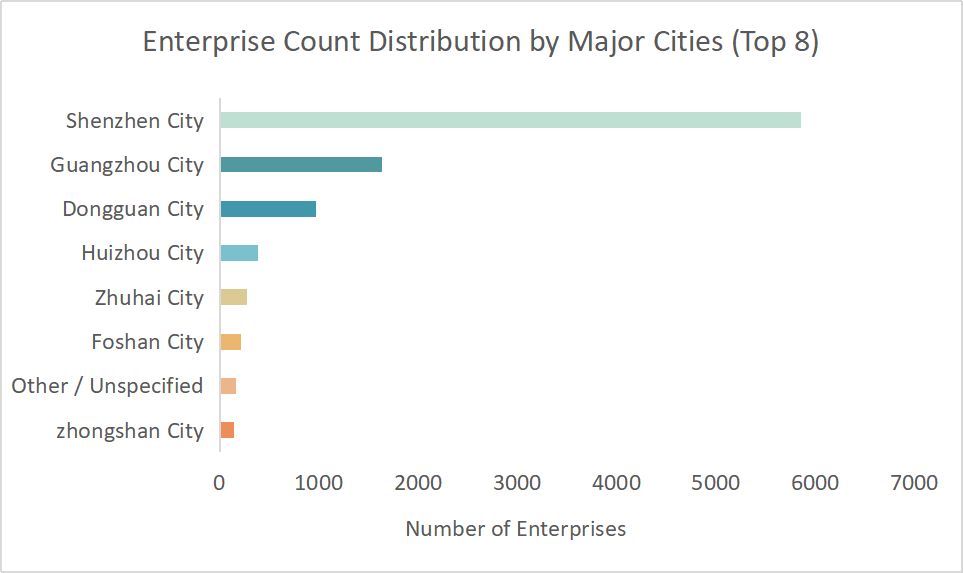
\includegraphics[width=\textwidth]{ent_dist_by_city.png}
\caption{Enterprise Count Distribution by Major Cities}
\label{fig:city_dist}
\end{figure}


\textbf{Key finding:} The top four cities (Shenzhen, Guangzhou, Dongguan, Huizhou)
account for 89.2\% of all enterprises, forming a ``Shenzhen as core, PRD as hinterland''
pattern. Eastern and northern Guangdong have negligible presence (Chaozhou: 3 firms;
Yunfu: 4 firms), indicating that industrial spillover has yet to materialize.

% ---------- Table 3: City x Scale Cross-tabulation ----------
\begin{table}[H]
\centering
\small
\caption{Enterprise Scale Distribution by Major City}
\label{tab:city_scale}
\begin{tabular}{lrrrrrr}
\toprule
\tableHeaderRow
\textbf{City} & \textbf{XS(Micro)} & \textbf{S(Small)} & \textbf{M(Medium)} & \textbf{L(Large)} & \textbf{Unspec.} & \textbf{Total} \\
\midrule
\tableOddRow  Shenzhen   & 3,846 & 1,712 & 169 & 21 & 138 & 5,886 \\
\tableEvenRow Guangzhou  & 499   & 1,095 & 33  & 3  & 6   & 1,636 \\
\tableOddRow  Dongguan   & 814   & 133   & 7   & 4  & 11  & 969  \\
\tableEvenRow Huizhou    & 335   & 83    & 8   & 2  & 3   & 431  \\
\tableOddRow  Zhuhai     & 141   & 109   & 14  & 5  & 15  & 284  \\
\tableEvenRow Foshan     & 162   & 38    & 4   & 1  & 4   & 209  \\
\midrule
\tableOddRow  \textbf{Total} & \textbf{5,797} & \textbf{3,170} & \textbf{235} & \textbf{36} & \textbf{177} & \textbf{10,000} \\
\bottomrule
\end{tabular}
\end{table}

\textbf{Key finding:} Guangzhou has the healthiest scale structure (S-type: 66.9\%),
while Dongguan (XS-type: 84.0\%) and Huizhou (XS-type: 77.7\%) are dominated by
micro-enterprises, reflecting divergent positions in the value chain.


% ---------- Table 4: City x Industry ----------
\begin{table}[H]
\centering
\small
\caption{Industry Segment Distribution by Major City}
\label{tab:city_industry}
\begin{tabular}{lrrrr}
\toprule
\tableHeaderRow
\textbf{City} & \textbf{IC Design} & \textbf{IC Manufacturing} & \textbf{Total} & \textbf{Mfg. Share (\%)} \\
\midrule
\tableOddRow  Shenzhen   & 3,802 & 2,084 & 5,886 & 35.4 \\
\tableEvenRow Guangzhou  & 1,602 & 34    & 1,636 & 2.1  \\
\tableOddRow  Dongguan   & 832   & 137   & 969   & 14.1 \\
\tableEvenRow Huizhou    & 366   & 65    & 431   & 15.1 \\
\tableOddRow  Zhuhai     & 200   & 84    & 284   & 29.6 \\
\tableEvenRow Foshan     & 165   & 44    & 209   & 21.1 \\
\midrule
\tableOddRow  \textbf{Total} & \textbf{7,403} & \textbf{2,597} & \textbf{10,000} & \textbf{26.0} \\
\bottomrule
\end{tabular}
\end{table}

\textbf{Key finding:} Design firms dominate; Guangzhou is almost entirely design-focused
(only 34 manufacturing firms, 2.1\%). Shenzhen has the highest manufacturing share (35.4\%)
and is the city with manufacturing scale advantages.

% ---------- Table 5: Registered Capital ----------
\begin{table}[H]
\centering
\caption{Registered Capital Distribution}
\label{tab:capital}
\begin{tabular}{lrrrl}
\toprule
\tableHeaderRow
\textbf{Capital Range} & \textbf{Count} & \textbf{Share (\%)} & \textbf{Cum. (\%)} & \textbf{Top City} \\
\midrule
\tableOddRow  $<$0.1M RMB       & 1,671 & 16.7 & 16.7 & Shenzhen, Dongguan \\
\tableEvenRow 0.1--0.5M RMB     & 1,386 & 13.9 & 30.6 & Shenzhen, Guangzhou \\
\tableOddRow  0.5--1M RMB       & 2,516 & 25.2 & 55.7 & Shenzhen, Guangzhou \\
\tableEvenRow 1--5M RMB         & 2,412 & 24.1 & 79.8 & Shenzhen, Guangzhou \\
\tableOddRow  5--10M RMB        & 1,101 & 11.0 & 90.8 & Shenzhen, Guangzhou \\
\tableEvenRow 10--50M RMB       & 541   & 5.4  & 96.3 & Shenzhen \\
\tableOddRow  50--100M RMB      & 92    & 0.9  & 97.2 & Shenzhen \\
\tableEvenRow $>$100M RMB       & 80    & 0.8  & 98.0 & Shenzhen \\
\tableOddRow  Unparseable       & 201   & 2.0  & 100.0 & --- \\
\midrule
\tableEvenRow \textbf{Total}    & \textbf{10,000} & \textbf{100.0} & --- & --- \\
\bottomrule
\end{tabular}
\end{table}

\begin{table}[H]
\centering
\caption{Registered Capital Descriptive Statistics}
\label{tab:capital_stat}
\begin{tabular}{lrlr}
\toprule
\tableHeaderRow
\textbf{Statistic} & \textbf{Value} & \textbf{Statistic} & \textbf{Value} \\
\midrule
\tableOddRow  Valid sample   & 9,799 firms & Std.\ dev.       & RMB 192.11M \\
\tableEvenRow Median         & RMB 1M      & Min              & RMB 0 \\
\tableOddRow  Mean           & RMB 11.65M  & Max              & RMB 15B \\
\tableEvenRow 25th percentile & RMB 0.5M   & Skewness         & Right-skewed \\
\tableOddRow  75th percentile & RMB 5M     & Share $>$100M RMB & 0.8\% \\
\bottomrule
\end{tabular}
\end{table}

\textbf{Key finding:} The registered capital distribution is heavily right-skewed
(median RMB 1M vs.\ mean RMB 11.65M). Eight of the top 10 highest-capital firms
are manufacturing enterprises, all located in Shenzhen.

% ---------- Table 6: Top 10 by Registered Capital ----------
\begin{table}[H]
\centering
\small
\caption{Top 10 Enterprises by Registered Capital}
\label{tab:capital_top10}
\begin{tabular}{llrlrl}
\toprule
\tableHeaderRow
\textbf{Rank} & \textbf{Enterprise} & \textbf{City} & \textbf{Capital} & \textbf{Segment} & \textbf{Scale} \\
\midrule
\tableOddRow  1  & Runpeng Semiconductor (Shenzhen)      & Shenzhen & RMB 15.00B  & Mfg. & M \\
\tableEvenRow 2  & Pengxin Micro IC Manufacturing        & Shenzhen & RMB 7.13B   & Mfg. & L \\
\tableOddRow  3  & China Resources Micro (Shenzhen)      & Shenzhen & RMB 5.70B   & Mfg. & XS \\
\tableEvenRow 4  & Shenzhen Shengweixu Technology        & Shenzhen & RMB 5.00B   & Mfg. & S \\
\tableOddRow  5  & SMIC (Shenzhen)                       & Shenzhen & US\$2.42B   & Mfg. & L \\
\tableEvenRow 6  & Dongguan Feite Semiconductor Holding  & Dongguan & RMB 2.37B   & Mfg. & S \\
\tableOddRow  7  & Shenzhen Pengjin High-Tech            & Shenzhen & RMB 2.11B   & Mfg. & S \\
\tableEvenRow 8  & Silex Microsystems (Shenzhen)         & Shenzhen & RMB 1.50B   & Mfg. & S \\
\tableOddRow  9  & Zhuhai Chongda Circuit Technology     & Zhuhai   & RMB 1.30B   & Design & L \\
\tableEvenRow 10 & Huatong Precision (Huizhou)            & Huizhou  & RMB 1.28B   & Mfg. & L \\
\bottomrule
\end{tabular}
\end{table}

% ---------- Table 7: Incorporation Timeline ----------
\begin{table}[H]
\centering
\small
\caption{New Enterprise Incorporation by Year (2017--2026)}
\label{tab:established}
\begin{tabular}{lrrrrr}
\toprule
\tableHeaderRow
\textbf{Year} & \textbf{IC Design} & \textbf{IC Mfg.} & \textbf{Total} & \textbf{Mfg. Share (\%)} & \textbf{YoY Change} \\
\midrule
\tableOddRow  2017 & 306 & 75  & 381  & 19.7 & ---      \\
\tableEvenRow 2018 & 481 & 95  & 576  & 16.5 & +51.2\%  \\
\tableOddRow  \textbf{2019} & \textbf{1,515} & \textbf{108} & \textbf{1,623} & \textbf{6.7} & \textbf{+181.8\%} \\
\tableEvenRow 2020 & 666 & 114 & 780  & 14.6 & $-$51.9\% \\
\tableOddRow  \textbf{2021} & \textbf{1,329} & \textbf{175} & \textbf{1,504} & \textbf{11.6} & \textbf{+92.8\%} \\
\tableEvenRow 2022 & 928 & 216 & 1,144 & 18.9 & $-$23.9\% \\
\tableOddRow  2023 & 504 & 269 & 773  & 34.8 & $-$32.4\% \\
\tableEvenRow 2024 & 462 & 266 & 728  & 36.5 & $-$5.8\%  \\
\tableOddRow  2025 & 723 & 331 & 1,054 & 31.4 & +44.8\%  \\
\tableEvenRow 2026 & 234 & 136 & 370  & 36.8 & ---      \\
\midrule
\tableOddRow  \textbf{Total} & \textbf{7,148} & \textbf{1,850} & \textbf{8,998} & \textbf{20.6} & --- \\
\bottomrule
\end{tabular}
\end{table}

\textbf{Key finding:} Two peaks in 2019 and 2021 coincide with national and provincial
IC policy rollouts. The manufacturing share rose from 6.7\% in 2019 to 36.8\% in 2026,
indicating a structural shift from a ``design rush'' toward a more balanced mix.

% ---------- Table 8: Insured Employees ----------
\begin{table}[H]
\centering
\caption{Insured Employee Count Distribution}
\label{tab:insurance}
\begin{tabular}{lrrr}
\toprule
\tableHeaderRow
\textbf{Insured Employees} & \textbf{Firms} & \textbf{Share (\%)} & \textbf{Cum. (\%)} \\
\midrule
\tableOddRow  0           & 6,761 & 67.6 & 67.6  \\
\tableEvenRow 1--5        & 1,942 & 19.4 & 87.0  \\
\tableOddRow  6--10       & 431   & 4.3  & 91.3  \\
\tableEvenRow 11--20      & 321   & 3.2  & 94.5  \\
\tableOddRow  21--50      & 263   & 2.6  & 97.2  \\
\tableEvenRow 51--100     & 121   & 1.2  & 98.4  \\
\tableOddRow  101--200    & 69    & 0.7  & 99.1  \\
\tableEvenRow 201--500    & 53    & 0.5  & 99.6  \\
\tableOddRow  501--1000   & 17    & 0.2  & 99.7  \\
\tableEvenRow $>$1000     & 22    & 0.2  & 100.0 \\
\midrule
\tableOddRow  \textbf{Total} & \textbf{10,000} & \textbf{100.0} & --- \\
\bottomrule
\end{tabular}
\end{table}

\textbf{Key finding:} Over two-thirds of enterprises have zero insured employees,
suggesting many are shell companies or pre-operational start-ups. Among the 3,239 firms
with positive insurance records, the median headcount is only 4, further confirming
the micro-enterprise character of the industry.

% ---------- Table 9: Enterprise Type ----------
\begin{table}[H]
\centering
\caption{Enterprise Ownership Type Distribution}
\label{tab:enterprise_type}
\begin{tabular}{lrrr}
\toprule
\tableHeaderRow
\textbf{Enterprise Type} & \textbf{Count} & \textbf{Share (\%)} & \textbf{Cum. (\%)} \\
\midrule
\tableOddRow  LLC (sole natural person)           & 3,087 & 30.9 & 30.9 \\
\tableEvenRow LLC                                  & 2,829 & 28.3 & 59.2 \\
\tableOddRow  LLC (natural person investment)      & 2,382 & 23.8 & 83.0 \\
\tableEvenRow LLC (sole legal person)              & 414   & 4.1  & 87.1 \\
\tableOddRow  Other LLC                            & 206   & 2.1  & 89.2 \\
\tableEvenRow LLC (natural+legal person investment) & 157  & 1.6  & 90.8 \\
\tableOddRow  Limited partnership                  & 153   & 1.5  & 92.3 \\
\tableEvenRow HK/Macau/foreign-funded (combined)   & 291   & 2.9  & 95.2 \\
\tableOddRow  Sole proprietorship / other          & 481   & 4.8  & 100.0 \\
\midrule
\tableEvenRow \textbf{Total} & \textbf{10,000} & \textbf{100.0} & --- \\
\bottomrule
\end{tabular}
\end{table}


\textbf{Key finding:} Private enterprises dominate (sole natural person + natural person
investment = 54.7\%); foreign participation is minimal (2.9\%), indicating that
Guangdong's IC industry is predominantly domestically driven with limited FDI spillovers.


\subsection{Output Data (2023--2025)}
\label{sec:output}

Annual output value, growth rates, sub-sector shares, and supporting
indicators for Guangdong's IC industry from 2023 to 2025. As of
May 2026, the province-wide total output value for 2025 has not yet
been released; however, IC output volume, exports, and imports for
2025 are available (Table~\ref{tab:core}), along with broader
industry indicators in the supplementary data tables. Additional
metrics are archived in \texttt{data/guangdong\_ic\_output\_data.json}.

\begin{table}[H]
\centering
\caption{Guangdong IC Industry Output Value and Growth (2019--2024)}
\label{tab:core}
\begin{tabular}{lrr}
\toprule
\tableHeaderRow
\textbf{Year} & \textbf{Output (RMB~100M)} & \textbf{Growth (\%)} \\
\midrule
\tableOddRow  2019 & 1200 & --- \\
\tableEvenRow 2022 & 2200 & ---\textsuperscript{a} \\
\tableOddRow  2023 & $>$2700\textsuperscript{b} & $\approx$22.7\textsuperscript{c} \\
\tableEvenRow 2024 & 3604.16 & $\approx$33.5\textsuperscript{c} \\
\bottomrule
\end{tabular}

\vspace{2pt}
{\footnotesize
\textsuperscript{a} 2019--2022 CAGR $\approx$22.4\%, consistent with the government
target of $>$22\% annual growth.
\textsuperscript{b} Minimum value; actual figure slightly higher.
\textsuperscript{c} Approximate, derived from adjacent years' output values; not
an officially published growth rate.

\textbf{Sources:} 2019 and 2022 -- Guangdong DRC / DSTI / DIT
\textit{Action Plan for Cultivating Semiconductor \& IC Strategic Emerging
Industry Clusters (2023--2025)}; 2023 -- China Commercial Industry Research
Institute; 2024 -- 21st Century Business Herald / Guangdong IC Industry
Association.}
\end{table}

\begin{table}[H]
\centering
\caption{Guangdong IC Industry Sub-sector Shares (2024)}
\label{tab:subsector2024}
\begin{tabular}{lrrr}
\toprule
\tableHeaderRow
\textbf{Segment} & \textbf{Value (RMB~100M)} & \textbf{Share (\%)} & \textbf{YoY Growth (\%)} \\
\midrule
\tableOddRow  IC Design & 2109 & 58.6 & 31.13 \\
\tableEvenRow IC Manufacturing & 92 & 2.6 & 101.58 \\
\tableOddRow  IC Packaging \& Testing & 795 & 22.1 & 14.93 \\
\tableEvenRow Equipment \& Materials & 608 & 16.9 & --- \\
\midrule
\tableOddRow  \textbf{Total} & \textbf{3604} & \textbf{100.0} & \textbf{$\approx$33.5} \\
\bottomrule
\end{tabular}

\vspace{2pt}
{\footnotesize
\textbf{Note:} Manufacturing accounts for only 2.6\% of the total, representing
the most prominent weak link, yet its 101.58\% YoY growth is the highest among
all segments. Equipment \& Materials is a combined category; separate growth
rates are not publicly available.

\textbf{Sources:} Sub-sector values -- SICA (Shenzhen Semiconductor \& IC Industry
Alliance) industry research report; growth rates -- 21st Century Business Herald
/ Guangdong IC Industry Association.}
\end{table}


\subsection{Industrial Foundation and Supporting Facilities}
\label{sec:infrastructure}

Guangdong's IC industry chain is anchored by a strong design segment (RMB~211 billion
in 2024), while manufacturing and materials represent catch-up areas. Major
manufacturing projects are scaling up rapidly: SMIC Shenzhen's 12-inch F16 line
and Yuexin Semiconductor (CanSemi) Phase III and IV are expanding capacity. By
end-2024, the monthly production capacity for 12-inch wafers in Guangdong
surpassed 100,000 pieces. Technology support is provided by high-level platforms
including Peng Cheng Laboratory and the GBA National Innovation Center, which
facilitate the translation of laboratory patents into commercial products for
automotive and AI applications.

% ============================================================
%  Chapter 3 — Industry Profile
% ============================================================
\section{Industry Profile}
\label{sec:industry}

\subsection{Scale Characteristics}
\label{sec:scale}

\begin{itemize}
    \item \textbf{Total Industrial Scale:} The total output value of the entire
    industrial chain reached 360.4 billion yuan in 2024, a year-on-year increase
    of 22.4\%, ranking firmly among the national first echelons. It is expected to
    exceed 450--500 billion yuan by 2026, maintaining rapid expansion. Driven by
    sustained high growth in recent years, the scale is expected to approach 600
    billion yuan by 2030.
    \item \textbf{Growth Momentum:} Output growth rates from 2023 to 2025 were
    5.2\% → 18.3\% → 21.0\%. By 2025, the industrial growth rate reached as
    high as 21\%, significantly higher than the national average of 11.2\%.
    It has led the country in growth rate for three consecutive years,
    demonstrating outstanding counter-cyclical resilience and growth momentum.
    \item \textbf{Capacity Expansion:} The monthly production capacity of 12-inch
    wafers is expected to reach 250,000--300,000 pieces by 2026. The output value
    of the wafer manufacturing sector grew by 102\%, becoming the fastest-growing
    segment of the entire industrial chain.
\end{itemize}


\subsection{Structural Characteristics}
\label{sec:structure2}

Behind the impressive scale and growth rate, Guangdong's integrated circuit
industry has not achieved balanced development across all segments, but presents
a distinct unbalanced structure of ``strong midstream, weak upstream, and dominant
design''. This pattern is both a concentrated reflection of Guangdong's industrial
advantages and a key direction for subsequent industrial upgrading.

\begin{figure}[H]
\centering
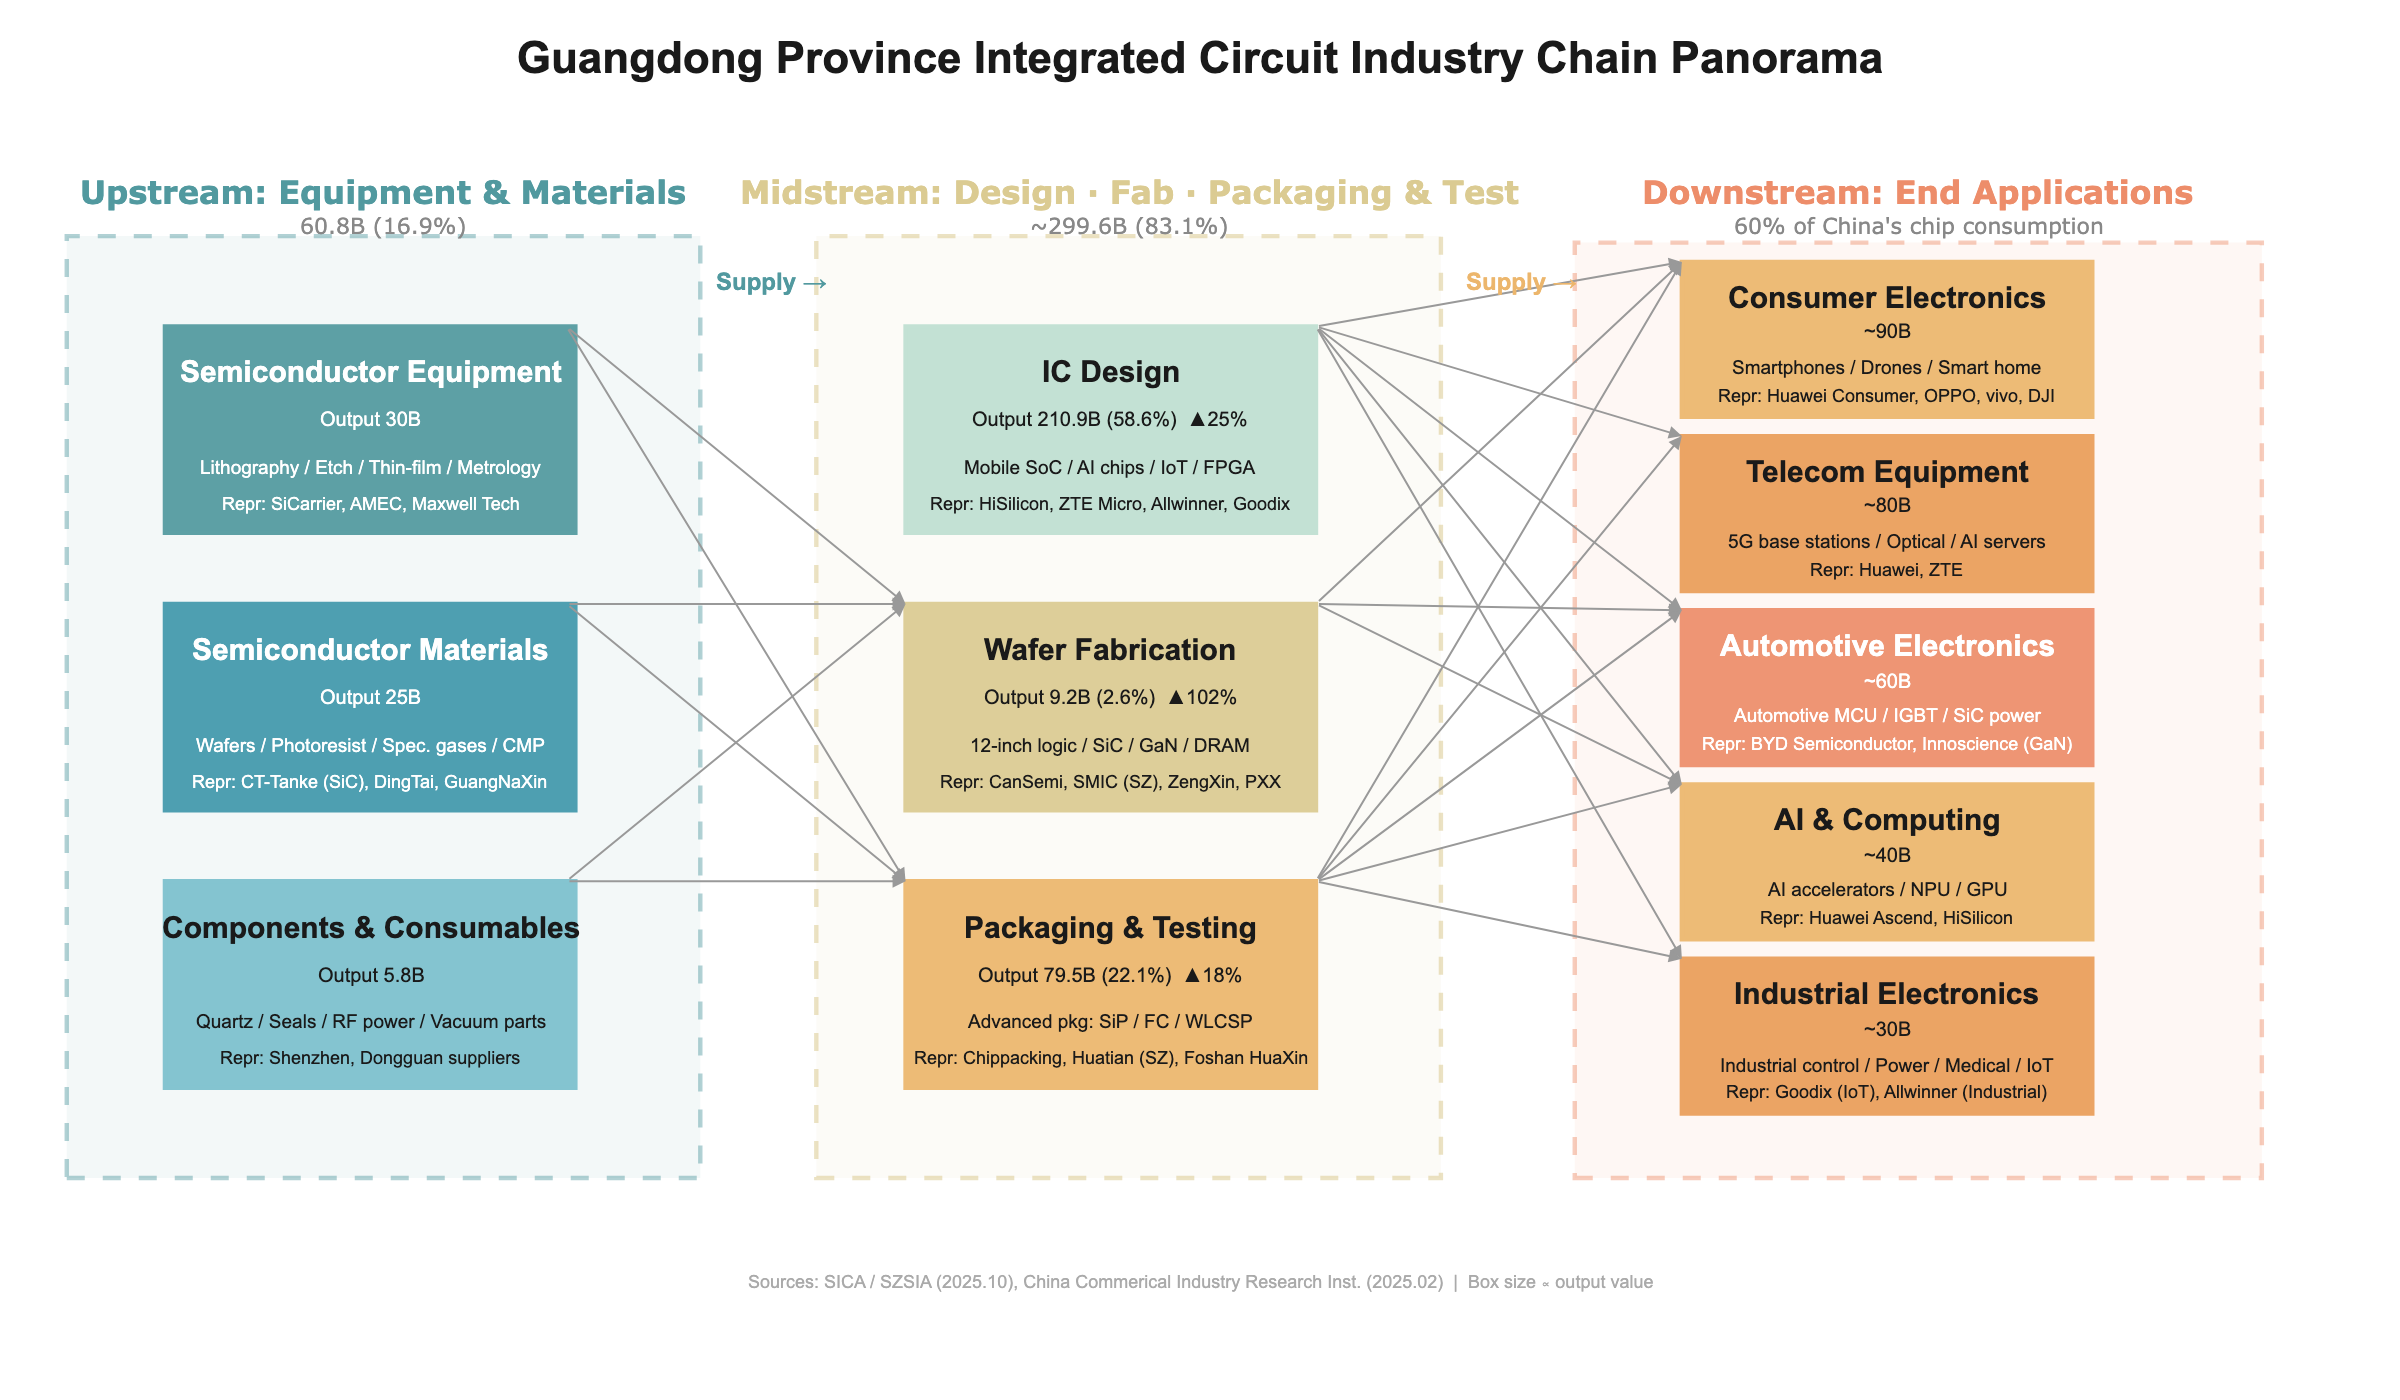
\includegraphics[width=\textwidth]{产业链全景图_EN.png}
\caption{Guangdong IC Industry Chain Panorama}
\label{fig:chain}
\end{figure}

\begin{itemize}
    \item \textbf{Core Advantage Segment:} IC design achieved an output value of
    210.9 billion yuan, accounting for 58.6\%, ranking first in China. Nanshan
    District of Shenzhen is a national hub for IC design, serving as the primary
    growth pole of the industry.
    \item \textbf{Stable Supporting Segment:} Packaging and testing achieved an
    output value of 79.5 billion yuan, accounting for 22.1\%. Mature packaging
    and testing clusters have been formed in Foshan and Zhongshan, with complete
    supporting capabilities.
    \item \textbf{Rapidly Catching-up Segment:} Wafer manufacturing achieved an
    output value of 9.2 billion yuan, accounting for only 2.6\%. Despite a small
    base, it has seen explosive growth, with projects such as Yuexin Semiconductor
    and SMIC Shenzhen ramping up production rapidly.
    \item \textbf{Obvious Weakness Segment:}Equipment and materials achieved an
    output value of 60.8 billion yuan, accounting for 16.9\%. Domestic substitution
    is still in an accelerated stage, representing the weakest part of the entire chain.
\end{itemize}

\subsection{Development Trends (2023--2025)}
\label{sec:development}

\subsubsection{Growth Trajectory and Cyclical Resilience}

Guangdong's IC industry has demonstrated outstanding counter-cyclical resilience
and growth momentum over the past three years, consistently outperforming the
national average:

\begin{table}[H]
\centering
\caption{Guangdong vs.\ National IC Output Growth Rate (2023--2025)}
\label{tab:growth_comparison}
\begin{tabular}{lrrr}
\toprule
\tableHeaderRow
\textbf{Year} & \textbf{Guangdong Growth (\%)} & \textbf{National Growth (\%)} & \textbf{Guangdong Premium} \\
\midrule
\tableOddRow  2023 & 5.2  & 3.0  & +2.2 pp \\
\tableEvenRow 2024 & 18.3 & 12.1 & +6.2 pp \\
\tableOddRow  \textbf{2025} & \textbf{21.0} & \textbf{11.2} & \textbf{+9.8 pp} \\
\bottomrule
\end{tabular}

\vspace{2pt}
{\footnotesize
\textbf{Sources:} AskCI 2025 Guangdong Semiconductor \& IC Industrial Chain
Panorama Report; Department of Industry and Information Technology of Guangdong
Province.}
\end{table}

\textbf{Key findings:}
\begin{itemize}
    \item In 2023, affected by the global semiconductor downturn cycle, the
          national IC output growth rate was only 3.0\%, yet Guangdong reached
          5.2\%, demonstrating strong counter-cyclical resilience.
    \item In 2024, driven by booming AI and automotive electronics demand,
          Guangdong's growth rate surged to 18.3\%, leading the national
          average by over 6 percentage points — a clear recovery inflection point.
    \item By 2025, Guangdong's IC output achieved 21.0\% year-on-year growth,
          nearly double the national rate of 11.2\%, marking three consecutive
          years as the national growth leader.
\begin{figure}[H]
\centering
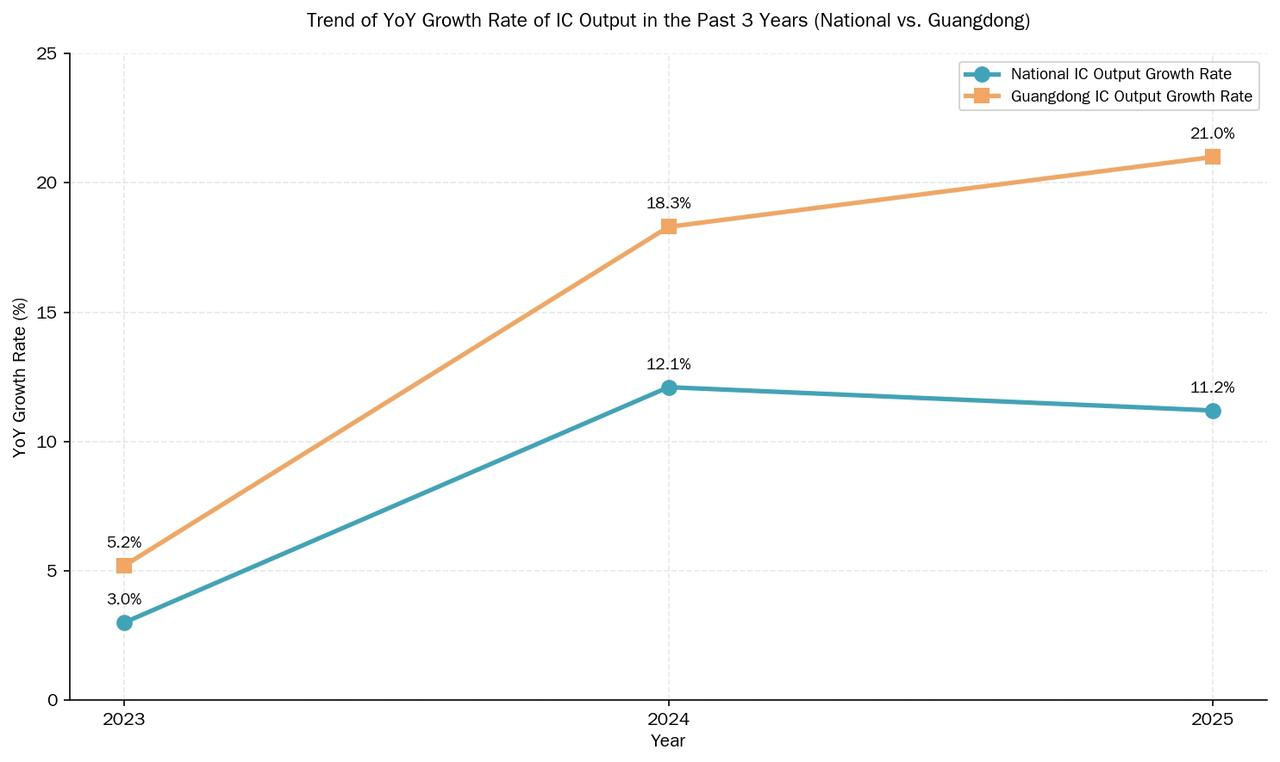
\includegraphics[width=\textwidth]{2023-2025IC产量同比增长_国际vs国内.jpeg}
\caption{IC Output YoY Growth: Guangdong vs.\ National (2023--2025)}
\label{fig:growth_comparison_chart}
\end{figure}

\end{itemize}

\subsubsection{Technology Evolution and Iteration}

The technological iteration of Guangdong's IC industry follows a pattern of
``design taking the lead, manufacturing achieving breakthroughs, and materials
keeping pace'':

\begin{enumerate}[label=(\arabic*)]
    \item \textbf{Design End:} AI chips, power semiconductors, and automotive
          electronic chips have become the focus of iteration. Products such
          as Huawei Ascend and HiSilicon Kirin have made key technological
          breakthroughs, and advanced process design capabilities continue to
          improve. The proportion of invention patents in the Greater Bay Area
          has risen from 28\% to 35.3\%, signaling structural upgrading of
          innovation quality.
    \item \textbf{Manufacturing End:} Wafer fabs represented by SMIC and
          Guangdong Yuexin Semiconductor (CanSemi) are steadily expanding
          production capacity. Mature process capacity continues to be released,
          and advanced packaging technologies such as SiP and Chiplet have made
          notable progress in Shenzhen and Guangzhou. Specifically, SiP has
          achieved large-scale commercial application in Shenzhen and is being
          deployed at a medium scale in Guangzhou, while Chiplet is still in the
          pilot and R\&D phase in both cities. The 12-inch wafer monthly capacity
          in Guangdong surpassed 100,000 pieces by end-2024 and is expected to
          reach 250,000--300,000 pieces by 2026.The manufacturing segment grew
          by 102\% in 2024, becoming the fastest-growing segment of the entire industrial chain.

    \item \textbf{Materials and Equipment:} Key domestic materials including
          photoresist, wet electronic chemicals, and target materials have
          realized local supporting supply in Guangdong, and some equipment
          enterprises have achieved domestic substitution of core components.
\begin{figure}[H]
\centering
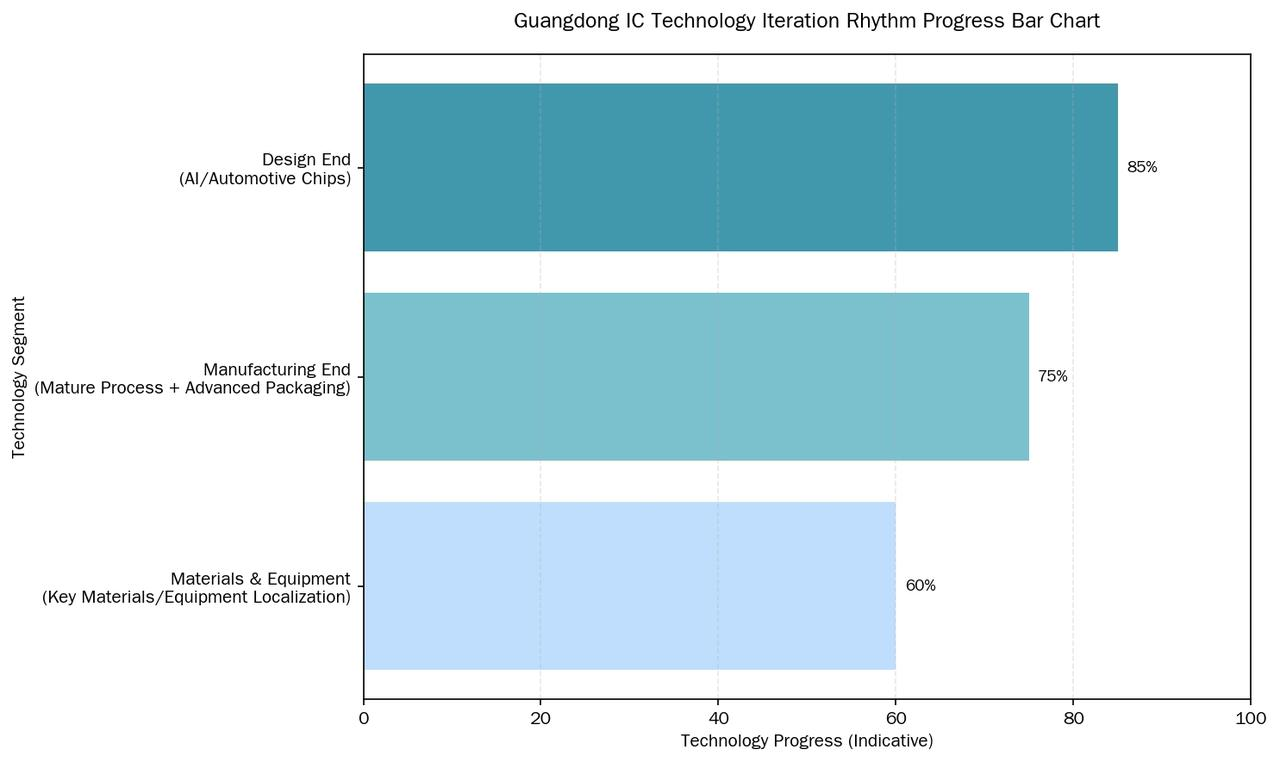
\includegraphics[width=\textwidth]{广东省IC技术迭代进度.jpeg}
\caption{Guangdong IC Technology Iteration Progress by Value Chain Segment}
\label{fig:tech_iteration}
\end{figure}

\end{enumerate}

\subsubsection{Key Pain Points}

Despite the impressive growth, several structural challenges persist:
(1) manufacturing and packaging/testing remain clear weaknesses relative to
design, with manufacturing accounting for only 2.6\% of total output value;
(2) advanced process bottlenecks below 7nm persist due to international
technology restrictions; (3) talent shortages — particularly in high-end
design, advanced manufacturing processes, and EDA — constrain further
expansion; and (4) the upstream equipment and materials segment remains the
weakest link in the value chain, with technological maturity estimated at
only 60\%.

\subsection{Key Indicator Framework}
\label{sec:indicators}

The following core indicators, derived from A-share semiconductor listed company
data compiled by JW Insights (Jiwei Network) and patent data from the Greater Bay
Area, provide a quantitative basis for assessing the innovation capability and
operational efficiency of Guangdong's IC industry.

\subsubsection{Core Indicator Trends (2023--2025)}

\begin{table}[H]
\centering
\small
\caption{Core Innovation and Efficiency Indicators (2023--2025)}
\label{tab:core_indicators}
\begin{tabular}{p{3cm}rrrp{3.2cm}}
\toprule
\tableHeaderRow
\textbf{Indicator} & \textbf{2023} & \textbf{2024} & \textbf{2025 (E)} & \textbf{Data Source} \\
\midrule
\tableOddRow  R\&D Investment Ratio (\%) & 12.12 & 10.66 & 10.5 & JW Insights A-share statistics \\
\tableEvenRow Semiconductor Patent Growth (\%) & 15.3 & 17.5 & 12.0 & Wisdom Bud GBA data \\
\tableOddRow  Capacity Utilization Rate (\%) & 82.0 & 84.8 & 93.0 & CanSemi (Yuexin) prospectus \\
\tableEvenRow Invention Patent Share (\%) & 28.0 & 31.5 & 35.3 & Wisdom Bud GBA data \\
\bottomrule
\end{tabular}

\vspace{2pt}
{\footnotesize
\textbf{Notes:} (1) R\&D investment ratio = R\&D expenditure / main business
revenue, based on A-share semiconductor listed company averages compiled by
JW Insights, used as a conservative benchmark for Guangdong Province (which,
with its high density of design enterprises, likely exceeds the national average).
(2) 2025 data are projected from Q1--Q3 actuals. (3) Capacity utilization rate
is based on CanSemi (Yuexin Semiconductor), the leading independent 12-inch
wafer foundry in Guangdong.
\begin{figure}[H]
\centering
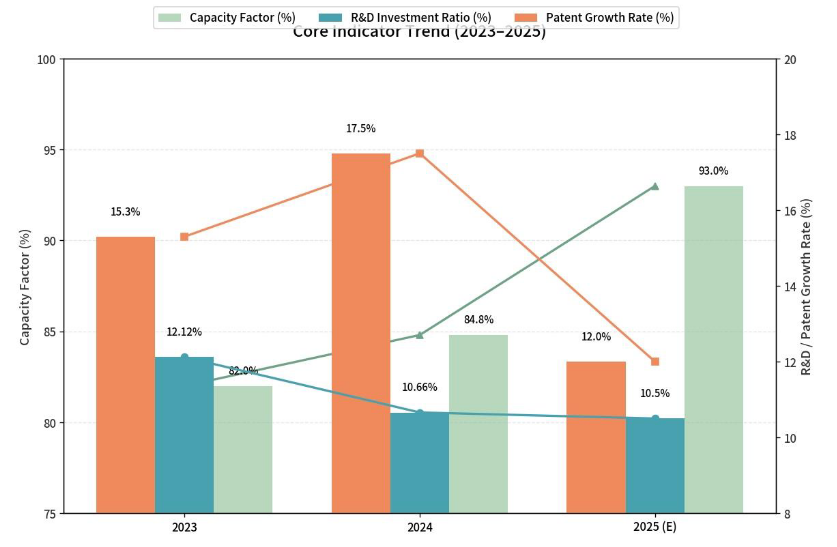
\includegraphics[width=\textwidth]{主要指标趋势.png}
\caption{Core Innovation and Efficiency Indicator Trends (2023--2025)}
\label{fig:indicator_trends}
\end{figure}
}
\end{table}

\subsubsection{Correlation Analysis: High Input $\rightarrow$ Strong Output $\rightarrow$ Rapid Conversion}

The three indicators exhibit a mutually reinforcing positive cycle:

\begin{enumerate}[label=(\arabic*)]
    \item \textbf{R\&D Investment $\rightarrow$ Patent Output:} The R\&D
          expenditure ratio for A-share semiconductor firms remains stably
          within the 10\%--12\% range, while semiconductor patents in the
          Greater Bay Area have seen a cumulative increase of approximately
          28\% over three years. R\&D investment is being steadily and
          consistently translated into accumulated intellectual property.
    \item \textbf{Patent $\rightarrow$ Capacity Absorption:} Patent quality
          has improved (the share of invention patents rose from 28\% to 35.3\%),
          production capacity utilization rose to 93\%, and the production-to-sales
          ratio reached 100\%. Technological achievements have entered a positive
          commercialization cycle.
    \item \textbf{Expense Ratio vs.\ Utilization Rate Interaction:} The expense
          ratio decreased from 12.12\% in 2023 to approximately 10.5\% in 2025,
          while the utilization rate rose from 82\% to 93\% over the same period.
          This ``passive dilution'' of the expense ratio is a positive signal:
          it was driven by substantial industry revenue growth (from approximately
          RMB 690 billion to RMB 882 billion), not by reduced R\&D intensity.
\end{enumerate}

\textbf{Core judgment:} A positive cycle has been established — R\&D investment
remains at a globally high level of over 10\%, patents continue to grow with
structural optimization, and production capacity operates at near-full capacity
with robust sales — all three elements functioning in synergy. The industry is
transitioning from large-scale expansion to a mature development phase
emphasizing both quality and efficiency.

\subsubsection{Technology Maturity by Segment}

{\footnotesize\textbf{Note:} The following technology maturity ratings are
qualitative assessments synthesized by the research group from industry reports
and expert interviews. They are intended for relative comparison across segments
rather than as precise quantitative metrics.}

\begin{table}[H]
\centering
\caption{Technology Maturity Assessment by Value Chain Segment}
\label{tab:tech_maturity}
\begin{tabular}{lrc}
\toprule
\tableHeaderRow
\textbf{Segment} & \textbf{Technology Maturity (\%)} & \textbf{Assessment} \\
\midrule
\tableOddRow  IC Design & 85 & Top-tier in China \\
\tableEvenRow IC Manufacturing & 75 & Steady breakthroughs \\
\tableOddRow  Packaging \& Testing & 75 & Steady breakthroughs \\
\tableEvenRow Equipment \& Materials & 60 & Prominent underlying technology gaps \\
\bottomrule
\end{tabular}
\end{table}

\subsubsection{Market Demand Structure}

Downstream applications are highly compatible with the province's three major
industrial layouts (traditional, emerging, and future industries):

\begin{itemize}
    \item \textbf{Empowering Traditional Industries:} Consumer electronics
          accounts for 35\% of IC demand, providing core support for the
          transformation and upgrading of home appliances and consumer
          electronics manufacturing.
    \item \textbf{Strengthening Emerging Industries:} Communications equipment
          and automotive electronics together account for 43\%, undertaking
          the main demand from 5G, new energy vehicles, and other emerging
          industries.
    \item \textbf{Layout for Future Industries:} Industrial control, AI servers,
          advanced computing, and other fields account for 22\%, seizing the
          technological and market high ground for future industries.
\begin{figure}[H]
\centering
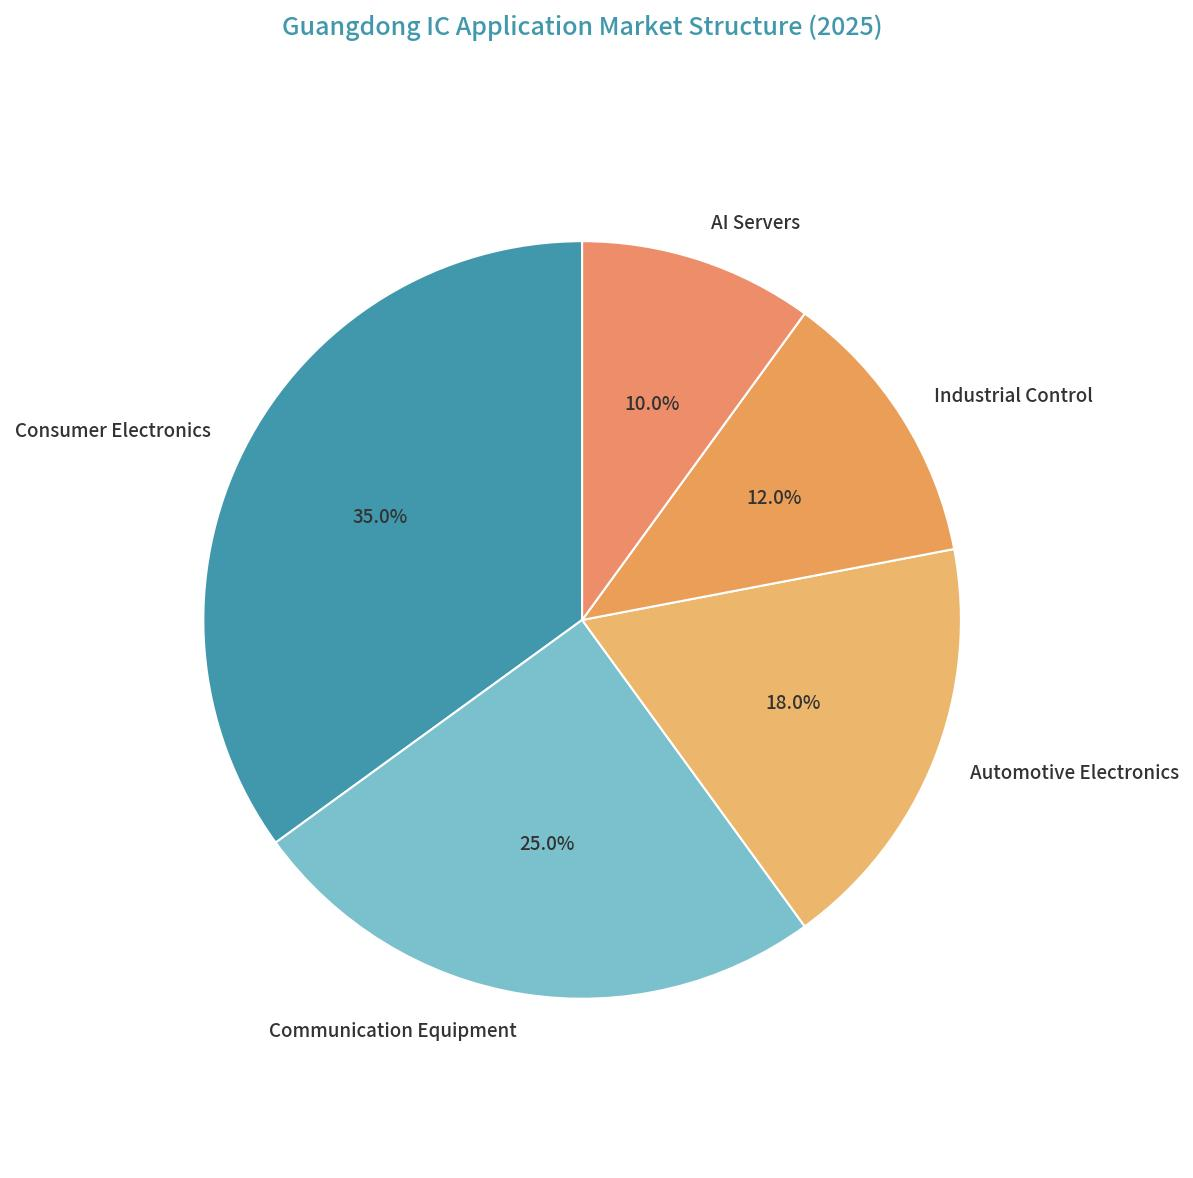
\includegraphics[width=\textwidth]{广东省IC产业应用市场结构.jpeg}
\caption{Guangdong IC Industry Downstream Application Market Structure}
\label{fig:app_market}
\end{figure}

\end{itemize}


\subsection{Market Structure and Concentration}
\label{sec:market_structure}

\subsubsection{Market Concentration (CR5/CR10/CR30)}

Market concentration analysis, based on registered capital of enterprises in
the Guangdong IC Enterprise Directory, reveals a highly oligopolistic market
structure:

\begin{table}[H]
\centering
\caption{Market Concentration Indices (Based on Registered Capital)}
\label{tab:concentration}
\begin{tabular}{lrrl}
\toprule
\tableHeaderRow
\textbf{Index} & \textbf{Share (\%)} & \textbf{Cumulative Capital (RMB 100M)} & \textbf{Interpretation} \\
\midrule
\tableOddRow  CR5  & 52.56 & 5,915.55 & Top 5 control over half of industry capital \\
\tableEvenRow CR10 & 67.15 & 7,556.72 & Top 10 control over two-thirds of capital \\
\tableOddRow  CR30 & 88.70 & ---     & Top 30 near-monopoly on capital resources \\
\bottomrule
\end{tabular}

\vspace{2pt}
{\footnotesize
\textbf{Note:} CR indices are calculated based on registered capital, not
operating revenue or market share, and reflect capital concentration
characteristics only.}
\end{table}

\textbf{Market structure judgment:} With a CR10 of 67.15\%, Guangdong's IC
industry exhibits a \textbf{high oligopolistic market structure} characterized
by: (1) market dominance highly concentrated in a small number of large
enterprises; (2) leading enterprises possessing absolute competitive advantages
in capital scale; and (3) extremely high capital barriers for new entrants.

This capital concentration coexists with a highly fragmented enterprise-count
distribution (95.3\% micro and small enterprises), producing a distinctive
``capital-concentrated, entity-fragmented'' dual structure: a small number of
capital-intensive manufacturing firms control the majority of financial
resources, while thousands of micro-design firms compete across a crowded
landscape with minimal capital endowments.
\begin{figure}[H]
\centering
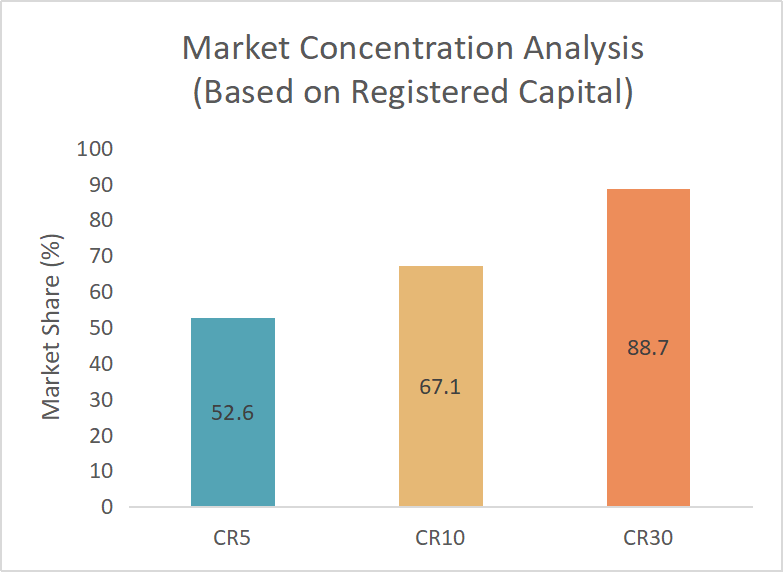
\includegraphics[width=\textwidth]{市场集中度分析.png}
\caption{Market Concentration Analysis (CR5/CR10/CR30 Based on Registered Capital)}
\label{fig:concentration_chart}
\end{figure}


\subsubsection{Enterprise Scale Structure}

The enterprise scale structure forms a pronounced pyramid shape:

\begin{table}[H]
\centering
\caption{Enterprise Type Structure by Scale Tier}
\label{tab:enterprise_tiers}
\begin{tabular}{lrrl}
\toprule
\tableHeaderRow
\textbf{Tier} & \textbf{Count} & \textbf{Share (\%)} & \textbf{Characteristics} \\
\midrule
\tableOddRow  SMEs (Micro + Small)     & 9,060 & 90.30 & Dominant in quantity, minimal capital scale \\
\tableEvenRow Above-scale enterprises  & 588   & 5.86  & Backbone of industrial support \\
\tableOddRow  Leading enterprises       & 385   & 3.84  & Smallest in number, control major capital \\
\bottomrule
\end{tabular}
\end{table}

This pyramid structure of ``SMEs as the foundation, above-scale enterprises as
the backbone, and a small number of leading enterprises'' indicates a solid
industrial ecosystem with substantial innovation vitality, but insufficient
industry leadership. The overall characteristics are ``large but not strong,
scattered but not concentrated,'' with broad room for integration and upgrading.

\subsubsection{Ownership Structure}

The ownership composition reveals a predominantly private-sector-driven industry:

\begin{itemize}
    \item \textbf{Private enterprises:} 75\%--80\%, serving as the main force
          of innovation and market development, concentrated in fabless design,
          AI chips, and automotive semiconductors.
    \item \textbf{State-owned enterprises:} 10\%--15\%, focusing on heavy-asset
          manufacturing including wafer fabrication, memory manufacturing, and
          industrial infrastructure.
    \item \textbf{Foreign-funded / joint ventures:} 5\%--10\%, supplementing
          capabilities in high-end manufacturing, advanced packaging/testing,
          EDA software, and semiconductor equipment.
\end{itemize}

This ownership pattern reflects the broader national industry structure:
private firms dominate innovation in AI chips and RISC-V architectures,
state-backed capital remains critical in wafer fabrication, and foreign firms
retain technological leadership in advanced equipment and EDA tools.

\subsubsection{Regional Capital Concentration}

Capital is even more spatially concentrated than enterprise counts:

\begin{table}[H]
\centering
\caption{Regional Distribution of Registered Capital (Top 3 Cities)}
\label{tab:capital_region}
\begin{tabular}{lrrl}
\toprule
\tableHeaderRow
\textbf{City} & \textbf{Capital (RMB 100M)} & \textbf{Share (\%)} & \textbf{Role} \\
\midrule
\tableOddRow  Shenzhen & 7,866.72 & 69.90 & Core capital agglomeration hub \\
\tableEvenRow Zhuhai   & 2,139.56 & 19.01 & Second largest capital scale \\
\tableOddRow  Jiangmen & 580.02   & 5.15  & Important capital node \\
\bottomrule
\end{tabular}
\end{table}

The nine Pearl River Delta cities collectively account for 95.64\% of
enterprises and 99.80\% of registered capital in the province, demonstrating
extreme spatial agglomeration. Non-PRD regions (eastern, western, and
northern Guangdong) are virtually absent from the IC capital landscape.
\begin{figure}[H]
\centering
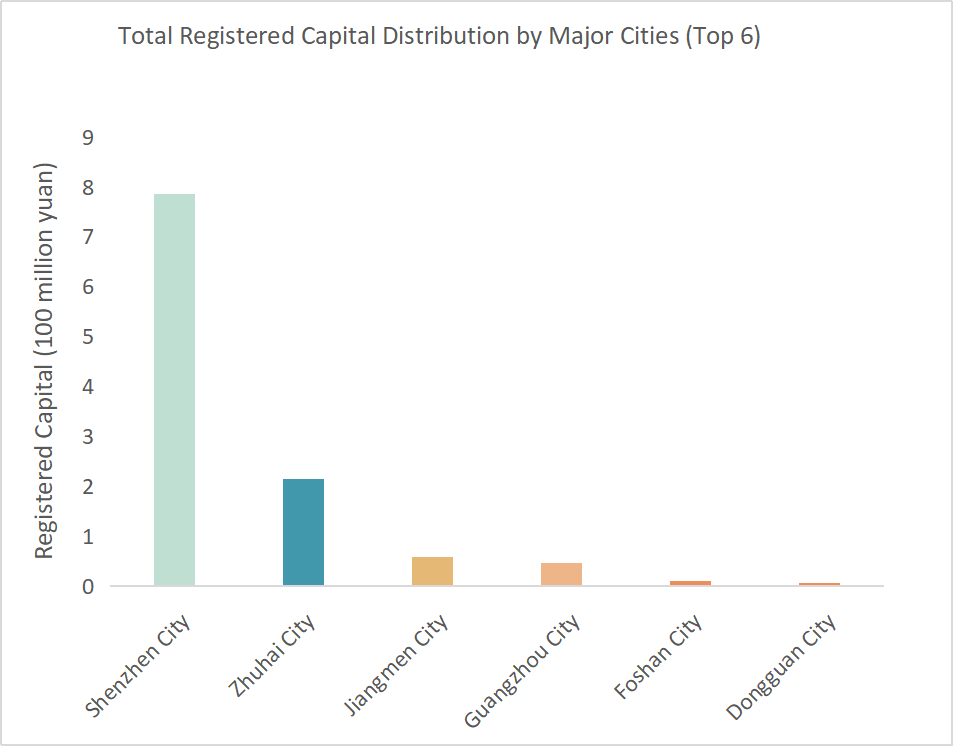
\includegraphics[width=\textwidth]{主要城市总注册资本分布.png}
\caption{Total Registered Capital Distribution by Major Cities}
\label{fig:capital_dist}
\end{figure}


\section{Talent Profile}
\label{sec:talent}

\subsection{Talent Scale and Composition}
\label{sec:talent_scale}

\subsubsection{Overall Talent Scale and Industrial Distribution}

Guangdong Province is one of China's three core IC industry clusters. The
industrial layout is centered on IC design, extended by specialty process
manufacturing, advanced packaging and testing, and compound semiconductors,
with synchronized development of supporting equipment and material enterprises.

{\footnotesize\textbf{Data note:} Talent figures in this subsection are based
on a sampling survey of over 2,000 major enterprises conducted by the Guangdong
Semiconductor Industry Association and represent estimates rather than official
government statistics. Numbers should be interpreted as indicative of relative
scale and structure rather than precise counts.}

The total number of employees in the province's entire IC industry chain is
estimated at approximately \textbf{236,000}, accounting for roughly 34\% of the
national IC workforce (approximately 630,000 nationally, per the China IC
Industry Talent White Paper 2020--2021), with talent agglomeration ranking
second in the country after the Yangtze River Delta.

Divided by industrial chain segments, the talent volume of each sector highly
matches the regional industrial positioning:

\begin{table}[H]
\centering
\caption{Talent Distribution by Value Chain Segment}
\label{tab:talent_segment}
\begin{tabular}{p{3.8cm}rrp{6.8cm}}
\toprule
\tableHeaderRow
\textbf{Segment} & \textbf{Employees} & \textbf{Share (\%)} & \textbf{Characteristics} \\
\midrule
\tableOddRow  IC Design & 172,000 & 72.9 & One of the most concentrated IC design talent pools in China \\
\tableEvenRow Wafer Manufacturing \& Specialty Processes & 28,000 & 11.9 & Smaller than Yangtze River Delta; expanding with new fabs \\
\tableOddRow  Packaging \& Testing & 24,000 & 10.2 & Concentrated in PRD manufacturing cities \\
\tableEvenRow Equipment, Materials, EDA \& IP Support & 12,000 & 5.1 & Supporting talent system still in cultivation stage \\
\midrule
\tableOddRow  \textbf{Total} & \textbf{236,000} & \textbf{100.0} & --- \\
\bottomrule
\end{tabular}
\end{table}

\textbf{Key finding:} IC design is the largest talent segment, accounting for
nearly three-quarters of the provincial IC workforce, reflecting Guangdong's
position as a national leader in fabless chip design. The manufacturing talent
pool remains undersized relative to the Yangtze River Delta, constraining the
province's capacity expansion ambitions.

The current explicit talent gap in the province's IC industry is approximately
\textbf{87,000}, with the largest gaps in high-end R\&D, advanced processes,
core IP, and EDA tools. With the continuous expansion of multiple 12-inch wafer
production lines and third-generation semiconductor production lines, total
talent demand is expected to exceed \textbf{300,000 by 2027}, and medium-to
long-term talent supply pressure will continue to intensify.

\subsubsection{Regional Talent Layout}

IC talents in Guangdong are characterized by high concentration and gradient
distribution, with core resources concentrated in the Pearl River Delta and
negligible presence in eastern, western, and northern Guangdong:

\begin{table}[H]
\centering
\caption{Regional Distribution of IC Talent in Guangdong}
\label{tab:talent_region}
\begin{tabular}{p{3.5cm}rrp{6.8cm}}
\toprule
\tableHeaderRow
\textbf{City/Region} & \textbf{Employees} & \textbf{Share (\%)} & \textbf{Industrial Focus} \\
\midrule
\tableOddRow  Shenzhen & 138,000 & 58.5 & Design hub: general chips, AI chips, power ICs, RF/analog \\
\tableEvenRow Guangzhou & 32,000 & 13.6 & Manufacturing core: wafer fab, specialty processes, R\&D institutes \\
\tableOddRow  Dongguan, Foshan, Zhongshan & 39,000 & 16.5 & Packaging/testing, discrete devices, component manufacturing \\
\tableEvenRow Zhuhai & 17,000 & 7.2 & Compound semiconductors, RF chips, industrial control IC design \\
\tableOddRow  Eastern, Western, Northern Guangdong & $<$10,000 & $<$4.2 & Minimal: only distribution and technical service roles \\
\midrule
\tableEvenRow \textbf{Total} & \textbf{236,000} & \textbf{100.0} & --- \\
\bottomrule
\end{tabular}
\end{table}

\textbf{Key finding:} Shenzhen alone accounts for 58.5\% of the province's IC
workforce, and the top four city clusters together account for over 95\%.
Non-PRD regions are virtually absent from the IC talent landscape, with R\&D
talents essentially nonexistent in those areas.

\begin{figure}[H]
\centering
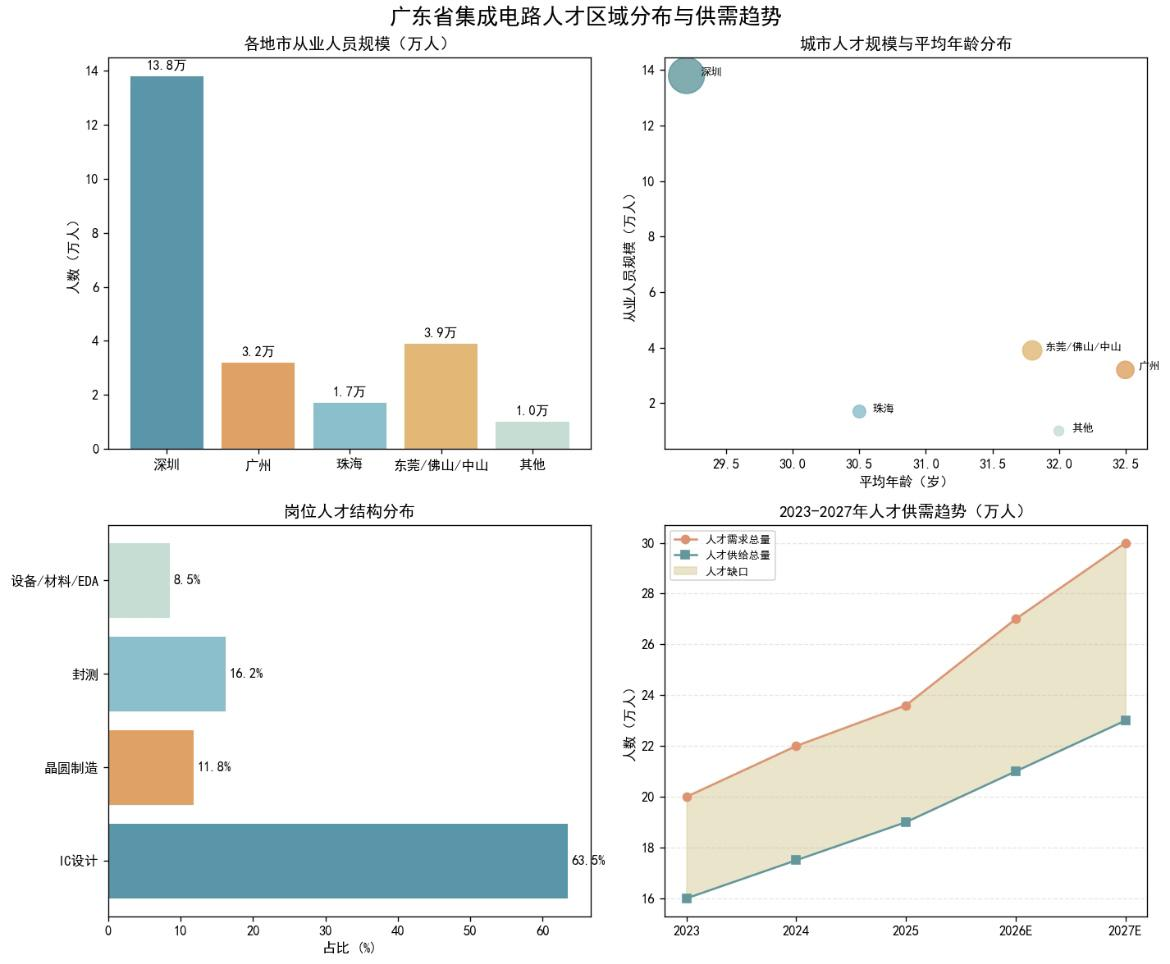
\includegraphics[width=\textwidth]{广东省集成电路人才区域分布与供需趋势.jpeg}
\caption{Guangdong IC Talent Regional Distribution and Supply-Demand Trends}
\label{fig:talent_region_chart}
\end{figure}

\subsubsection{Educational Background Structure}

Based on a sampling survey of over 2,000 major enterprises by the Guangdong
Semiconductor Industry Association, the educational attainment of IC
practitioners is significantly higher than the provincial manufacturing
average, with clear stratification by value chain segment:

\begin{table}[H]
\centering
\caption{Educational Attainment of IC Practitioners in Guangdong}
\label{tab:education}
\begin{tabular}{p{2.6cm}rp{2.5cm}p{7.2cm}}
\toprule
\tableHeaderRow
\textbf{Degree Level} & \textbf{Share (\%)} & \textbf{Est.\ Employees} & \textbf{Primary Roles} \\
\midrule
\tableOddRow  Doctoral & 3.3  & $\approx$7,790  & Advanced process R\&D, chip architecture, EDA algorithms, third-gen semiconductor materials \\
\tableEvenRow Master's & 36.8 & $\approx$86,800 & Core R\&D: IC design, process R\&D, chip verification, backend layout \\
\tableOddRow  Bachelor's & 37.1 & $\approx$87,500 & Testing, layout design, process execution, equipment maintenance, project management \\
\tableEvenRow Associate \& below & 22.8 & $\approx$53,900 & Production line operators, basic quality inspection, on-site auxiliary \\
\midrule
\tableOddRow  \textbf{Bachelor's+ subtotal} & \textbf{77.2} & \textbf{$\approx$182,000} & --- \\
\bottomrule
\end{tabular}
\end{table}

\textbf{Key findings:}
\begin{itemize}
    \item 77.2\% of employees hold a bachelor's degree or above, well above
          the provincial manufacturing average.
    \item Master's degree holders (36.8\%) form the main force in core R\&D
          positions; in Shenzhen and Guangzhou design enterprises, a master's
          degree has become the de facto entry threshold for core R\&D roles.
    \item Doctoral-level talent (3.3\%, approximately 7,790 people) is the most
          scarce group, concentrated in leading enterprise R\&D centers,
          universities, and research institutes.
    \item Educational stratification varies sharply by segment: over 90\%
          bachelor's+ in IC design enterprises, approximately 75\% in wafer
          manufacturing, and only approximately 55\% in packaging/testing.
\end{itemize}

\subsubsection{Professional Title Structure}

The title structure of the IC industry presents a typical pyramid shape with
a large base, under-pressure middle, and scarce top:

\begin{table}[H]
\centering
\caption{Professional Title Structure of IC Practitioners}
\label{tab:titles}
\begin{tabular}{p{4.5cm}rp{7.5cm}}
\toprule
\tableHeaderRow
\textbf{Title Level} & \textbf{Share (\%)} & \textbf{Characteristics} \\
\midrule
\tableOddRow  Junior (Assistant Engineer, Technician) & 49.6 & Fresh graduates and $<$3-year employees; most mobile group \\
\tableEvenRow Intermediate (Engineer) & 36.2 & 5--10 years of experience; core resource competed for by enterprises \\
\tableOddRow  Senior (Senior Engineer, Professor-level) & 10.5 & $>$10 years of experience; concentrated in leading enterprises \\
\tableEvenRow High-level Leading Talents \& Special Experts & 3.7 & Industrial leaders, provincial+ high-level talents; $<$1,000 people total \\
\bottomrule
\end{tabular}
\end{table}

\textbf{Key finding:} The proportion of senior technical personnel with more
than 15 years of working experience is critically low, making it difficult to
effectively inherit technical experience and process know-how. The total number
of high-level leading talents in the province is fewer than 1,000, representing
the core shortcoming restricting high-end industrial breakthroughs. Intermediate
engineers (the industry backbone) face continuous cross-regional talent loss
to the Yangtze River Delta due to salary and platform competition.

\subsubsection{Age Structure}

The IC industry in Guangdong is highly youthful, with a mean employee age of
\textbf{30.7 years}, lower than the national industry average. However, a
structural fault in senior technical talent is prominent:

\begin{itemize}
    \item \textbf{25--35 age group (57.3\%):} The absolute majority; strong
          learning ability and execution, but generally lacks full-process
          project experience in advanced nodes (7nm and below), large-scale
          complex SoC chips, and automotive-grade high-reliability chips.
    \item \textbf{35--45 age group (33.1\%):} Core technical backbone and
          grassroots management; complete project experience — but the total
          pool is small and subject to external poaching, creating an
          ``insufficient backbone layer'' problem in most enterprises.
    \item \textbf{45+ age group (9.6\%):} Senior technical experts and industry
          veterans with decades of accumulation; numbers cannot meet the needs
          of advanced production lines and cutting-edge R\&D, forming a
          structural contradiction of ``young teams with vitality but lack of
          experience, and senior talents with experience but small scale.''
\end{itemize}

In terms of regional differences, the mean age of design enterprise employees
in Shenzhen is the lowest at approximately 29.2 years, while manufacturing
and research enterprise employees in Guangzhou average approximately 32.5 years.

\subsection{Core Talent Demand}
\label{sec:talent_demand}

As Guangdong pivots from general technical workforce expansion toward overcoming
``bottleneck'' (\textit{ka bo zi}) technologies and achieving industrial
self-control, talent demand is undergoing a structural evolution — away from
general technicians toward multi-disciplinary professionals specialized in
advanced manufacturing, emerging applications, and digital transformation.

\subsubsection{Talent Demand by Industry Category}

\paragraph{Emerging Industries: Advanced Manufacturing and R\&D Talent.}
The explosive growth of new energy vehicles (NEVs), 5G, and AI computing has
made R\&D and manufacturing talent the most critical assets:

\begin{itemize}
    \item \textbf{Advanced Process Talent:} As technology nodes advance toward
          5nm, 3nm, and beyond, demand for Process/Yield Engineers (PE) has
          reached a peak, accounting for the highest demand share at 3.3\%
          of total IC job postings. These experts are essential for optimizing
          lithography, etching, and thin-film processes in mass production.
    \item \textbf{High-End Design Talent:} Analog IC Design and Digital
          Front-end Engineers are the core drivers of innovation. For AI chips,
          Algorithm Engineers are needed to optimize neural network models
          through hardware-friendly methods such as quantization and pruning.
\end{itemize}

\paragraph{Future Industries: Embodied Intelligence and Advanced Architecture.}
Forward-looking layouts in humanoid robotics and quantum computing demand
``forward-looking'' skill sets:

\begin{itemize}
    \item \textbf{AIoT and Embodied Intelligence:} The development of
          Industrial IoT (IIoT) drives demand for low-power, high-integration
          AIoT chips. Engineers must balance hardware computing power with
          software algorithms to achieve synergy between ``brain'' and ``body.''
    \item \textbf{Chiplet and Advanced Architecture:} As Moore's Law slows,
          Chiplet and Computing-in-Memory technologies are revolutionizing chip
          design. Architects must possess the ability to transcend traditional
          von Neumann bottlenecks to serve data centers and AI workloads.
\end{itemize}

\paragraph{Traditional Industries: Digital Transformation and Power Semiconductors.}
Traditional manufacturing's digital shift creates demand for embedded systems
and third-generation semiconductor applications:

\begin{itemize}
    \item \textbf{Digital Transformation Specialists:} Demand for Embedded
          Software Development and Driver Development remains stable (around
          2.1\% of job postings), as these professionals integrate IC
          technology into traditional equipment for connectivity and
          intelligence.
    \item \textbf{Third-Generation Semiconductors:} The penetration of Silicon
          Carbide (SiC) and Gallium Nitride (GaN) in NEVs and fast charging
          requires Material R\&D engineers with experience in high thermal
          stability and low-loss materials.
\end{itemize}

\subsubsection{Demand by Value Chain Segment}

Critical shortage occupations by value chain segment are summarized below:

\begin{table}[H]
\centering
\caption{Core Talent Shortage by Value Chain Segment}
\label{tab:talent_shortage}
\begin{tabular}{p{2.5cm}p{7cm}p{3.5cm}}
\toprule
\tableHeaderRow
\textbf{Segment} & \textbf{Key Shortage Positions} & \textbf{Severity} \\
\midrule
\tableOddRow  IC Design & Analog IC design, digital front-end/back-end, EDA software development, AI chip algorithm engineers & Highest shortage intensity \\
\tableEvenRow Wafer Manufacturing & Process R\&D engineers, lithography/etch/thin-film/ion implantation engineers, yield improvement engineers, production line integration engineers & Rapidly expanding gap \\
\tableOddRow  Packaging \& Testing & Advanced packaging R\&D (SiP/FC/WLCSP), Fan-out/2.5D/3D packaging engineers & Emerging direction; insufficient reserve \\
\tableEvenRow Equipment \& Materials & Semiconductor equipment R\&D, critical materials R\&D (photoresist, specialty gases, sputtering targets), EDA tool R\&D & Weakest link; $<$4,500 full-time EDA/IP professionals province-wide \\
\bottomrule
\end{tabular}
\end{table}

\subsubsection{Post Structure and Supply-Demand Characteristics}

Combined with the industrial chain format, the post structure has distinct
regional characteristics:

\begin{itemize}
    \item \textbf{IC Design Posts (63.5\% of total):} Digital IC design and
          chip verification have the strongest demand; analog/RF IC design
          and power management chip design are traditional advantageous posts
          with high talent thresholds and long training cycles, facing
          persistent long-term gaps. AI chip and automotive-grade chip design
          talent demand has grown fastest in the past three years.
    \item \textbf{Wafer Manufacturing and Process Posts (11.8\%):} With the
          implementation of multiple specialty process and third-generation
          semiconductor production lines, gaps in process engineers continue
          to expand. The manufacturing talent pool started late in Guangdong,
          and mature process engineers rely heavily on external introduction.
    \item \textbf{Packaging and Testing Posts (16.2\%):} Traditional packaging
          talent supply is adequate; Fan-out, 2.5D/3D advanced packaging
          represents an emerging direction with insufficient technical reserves.
    \item \textbf{Equipment, Materials, EDA \& IP Support (8.5\%):} The weakest
          link — fewer than 4,500 full-time EDA R\&D and IP development
          professionals province-wide; core tools and independent IP fields
          almost entirely rely on external talent introduction and procurement.
\end{itemize}

\subsubsection{Core Skills and Qualifications}

According to industry research, enterprises now emphasize a balance between
``hard tech'' and ``soft skills'':

\begin{itemize}
    \item \textbf{Professional Knowledge:} Solid foundation in Electronic
          Engineering, Microelectronics, Physics, and Mathematics; proficiency
          in EDA tools (Cadence, Synopsys) is mandatory.
    \item \textbf{Technical Depth:} RF Engineers must master high-frequency
          and miniaturized designs; Verification Engineers must be proficient
          in UVM architectures and FPGA prototyping.
    \item \textbf{Multi-disciplinarity:} With increasing SoC complexity,
          ``T-shaped'' talent with knowledge spanning Electronics, Computer
          Science, and Software is highly preferred.
    \item \textbf{Collaboration:} The ability to communicate effectively across
          the ``Design--Manufacturing--Testing'' chain is vital to ensure design
          accuracy and rapid yield ramp.
\end{itemize}

\subsubsection{Experience Preferences and Recruitment Characteristics}

Recruitment patterns show a clear ``action-oriented'' bias:

\begin{itemize}
    \item \textbf{Project Experience Priority:} Companies strongly prefer
          engineers with demonstrable project history who can immediately
          solve on-site problems such as yield improvement or failure analysis.
          Fresh graduates typically require 3--12 months of secondary training
          before independent assignment.
    \item \textbf{Mid-sized Firms Most Active:} Companies with 100--499
          employees are the primary recruiters (25.7\% of postings),
          reflecting their rapid expansion phase and urgent need for
          ``plug-and-play'' talent.
    \item \textbf{Cross-sector Talent Inflow:} While the IC industry primarily
          relies on internal talent flow, there is significant inflow from
          Machinery/Equipment (4.96\%), Internet (4.17\%), and Computer
          Software (4.05\%) sectors as technical skills become more transferable.
\end{itemize}

\subsection{Talent Distribution and Mobility}
\label{sec:talent_flow}

\subsubsection{Spatial Concentration and National Context}

China's IC talents are highly concentrated in three large urban agglomerations:
the Yangtze River Delta (Shanghai + Wuxi + Nanjing + Suzhou + Hangzhou + Hefei,
approximately 400,000 people), the Pearl River Delta (approximately 236,000 in
Guangdong Province), and the Beijing-Tianjin-Hebei region (Beijing + Tianjin,
approximately 140,000 people). Together, these three regions account for more
than 85\% of the national IC workforce (approximately 630,000 nationally).

Within this national landscape, Shanghai (approximately 200,000), Shenzhen
(approximately 138,000), and Beijing (approximately 130,000) form the first
tier, containing approximately 48\% of the national total.
\begin{figure}[H]
\centering
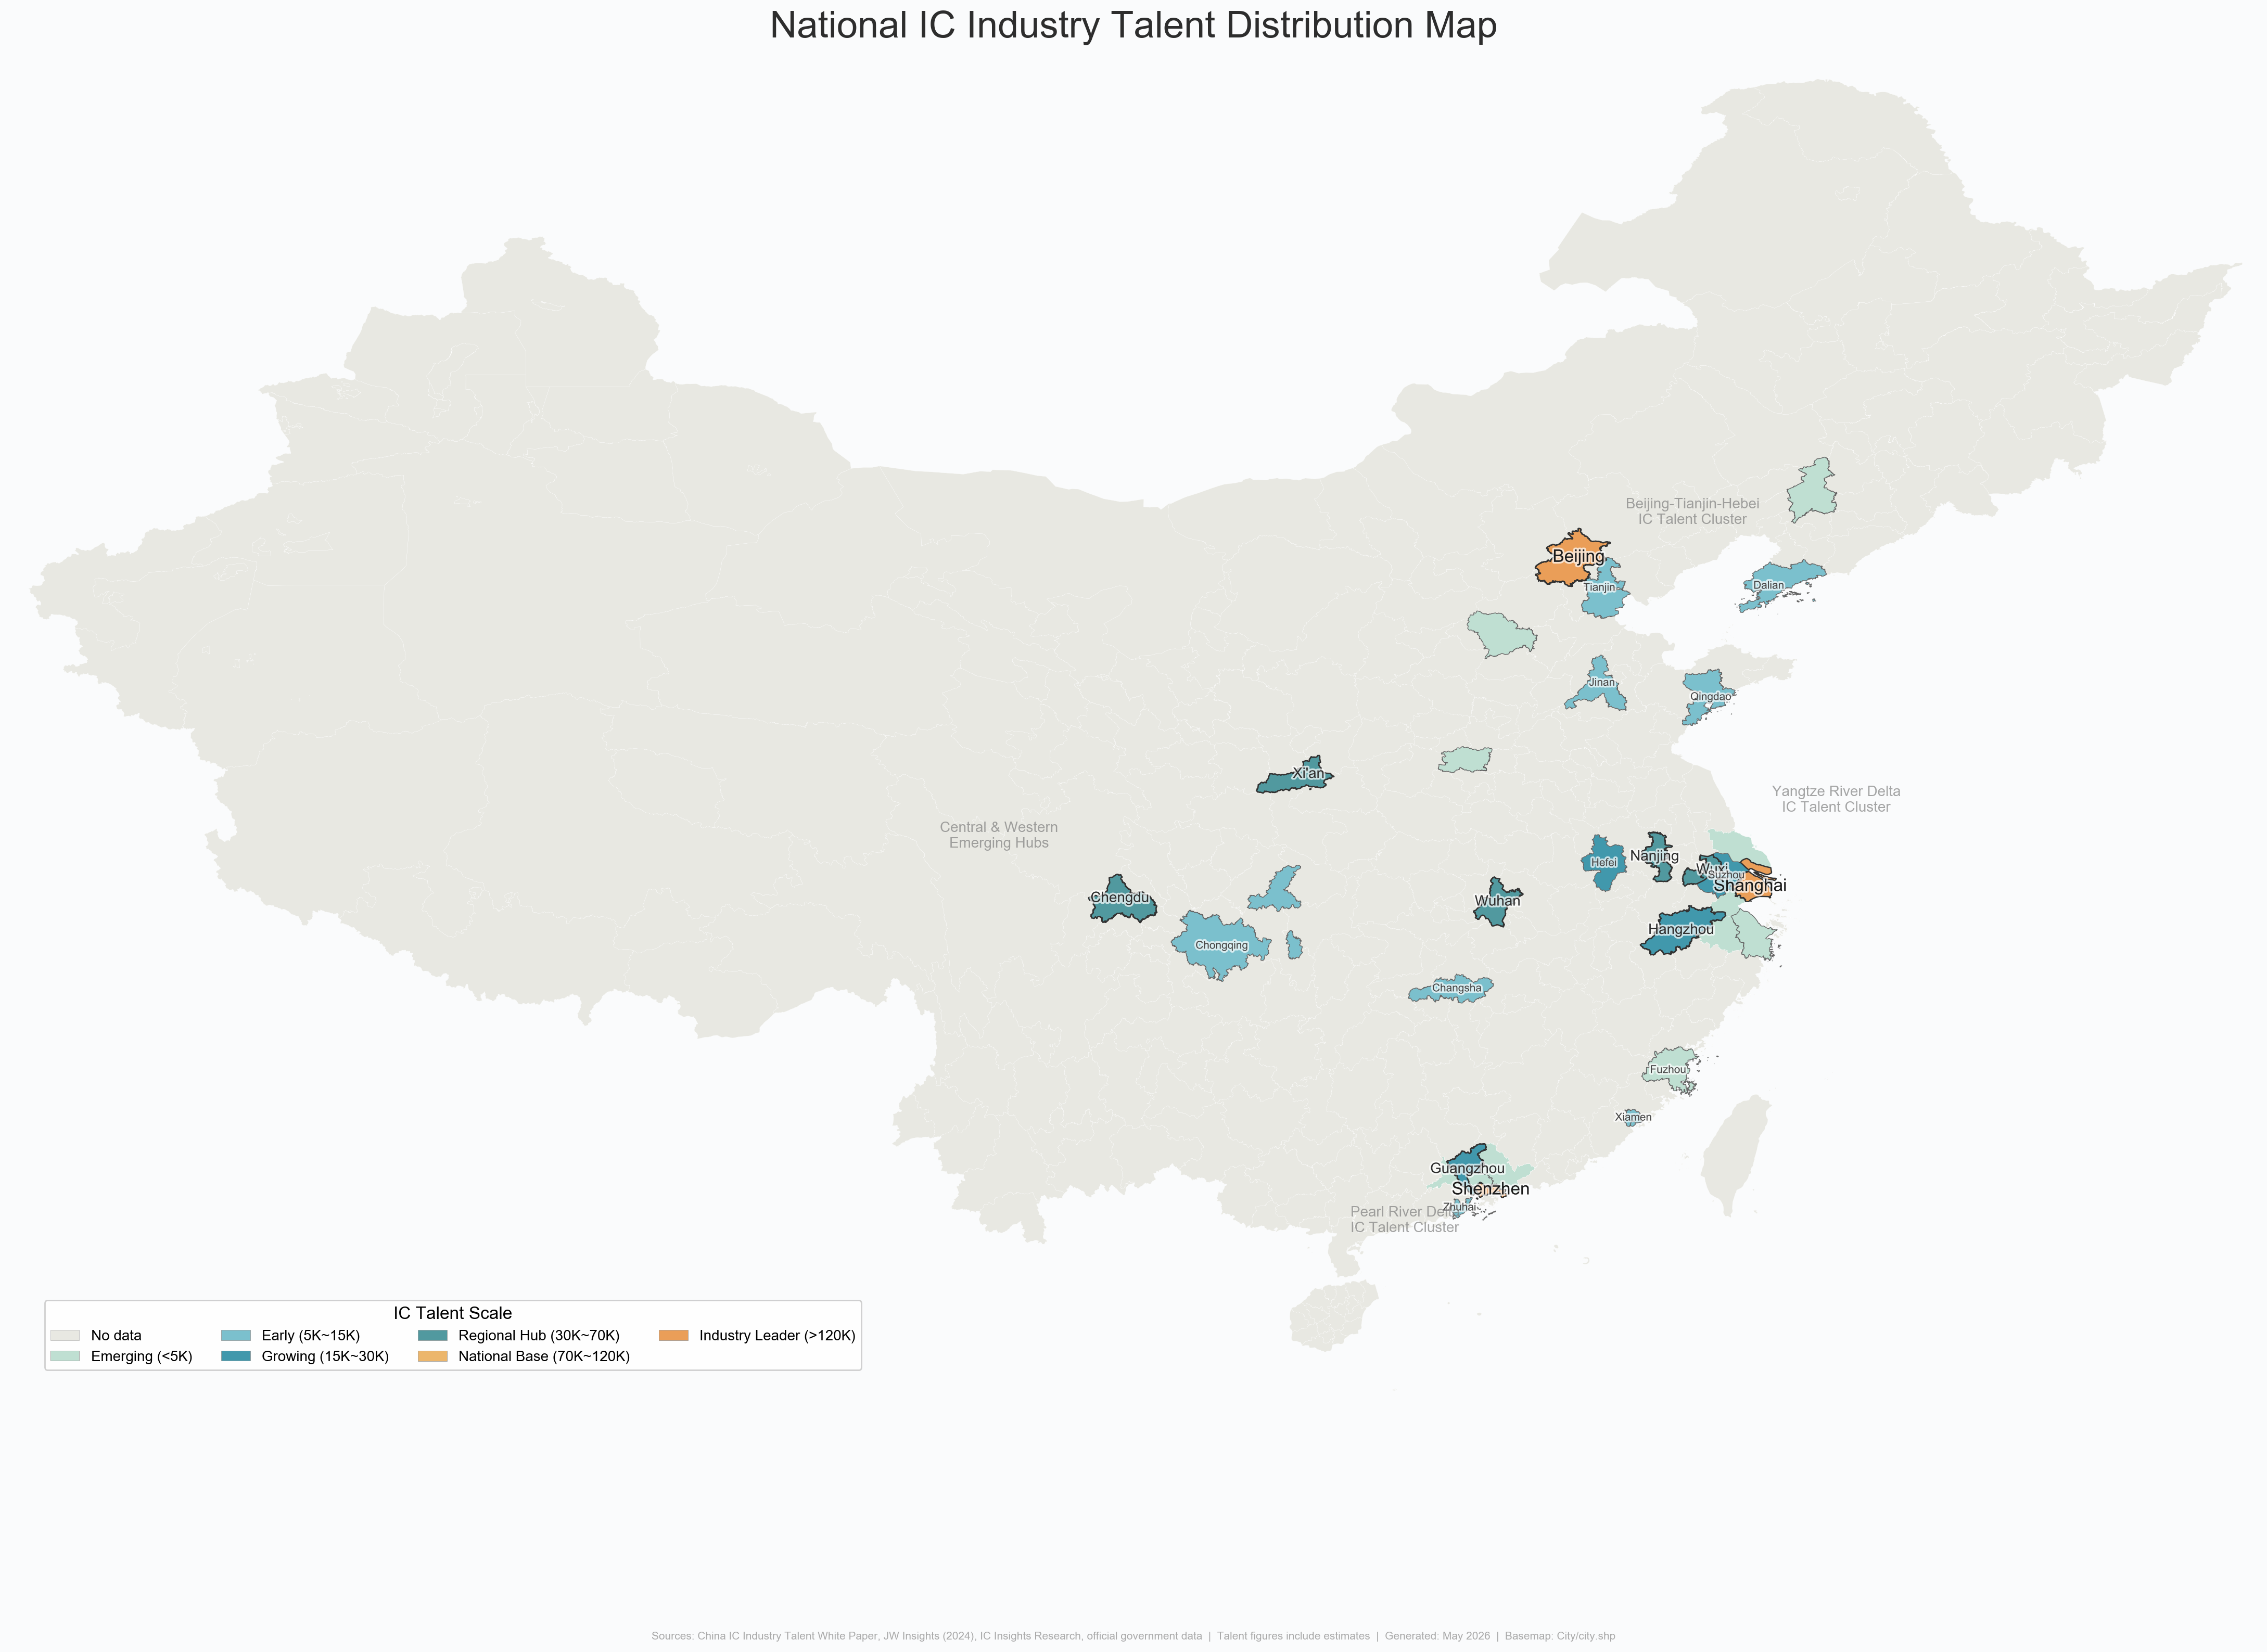
\includegraphics[width=\textwidth]{全国IC人才分布图_en.png}
\caption{National IC Industry Talent Distribution Map}
\label{fig:talent_map}
\end{figure}

\subsubsection{Intra-Provincial Mobility Patterns}

Bidirectional talent circulation among core PRD cities is documented by
commercial HR platform data (Liepin, 2024):

\begin{table}[H]
\centering
\caption{Talent Delivery Source Composition by City (Liepin 2024)}
\label{tab:talent_flow_cities}
\begin{tabular}{p{3.5cm}p{9.5cm}}
\toprule
\tableHeaderRow
\textbf{Delivery Destination} & \textbf{Top Sources (\% of total deliveries)} \\
\midrule
\tableOddRow  Guangzhou & Local 42.13\%, Shenzhen 8.17\%, Foshan 3.76\%, Dongguan 2.87\% \\
\tableEvenRow Shenzhen  & Local 37.58\%, Guangzhou 7.45\%, Shanghai 4.63\%, Beijing 3.86\% \\
\tableOddRow  Dongguan  & Local 27.46\%, Shenzhen 16.12\%, Guangzhou 8.91\% \\
\bottomrule
\end{tabular}

\vspace{2pt}
{\footnotesize
\textbf{Note:} Liepin platform data reflects voluntary job-seeking behavior
and is not equivalent to official government statistics; it is used here only
as a directional indicator of talent mobility patterns.}
\end{table}

\textbf{Key findings:}
\begin{itemize}
    \item Shenzhen exhibits strong talent retention (37.58\% local) but also
          significant outflows to Guangzhou, Shanghai, and Beijing, driven by
          competition for salaries, platforms, and living costs.
    \item Dongguan has the lowest local retention rate (27.46\%) and the
          highest dependence on Shenzhen (16.12\%), reflecting its role as a
          manufacturing hinterland receiving spillover from Shenzhen.
    \item Cross-sector inflow to the IC industry mainly originates from
          Electronics/Semiconductor/IC itself (7.86\%), followed by
          Machinery/Equipment (4.96\%), Internet (4.17\%), and Computer
          Software (4.05\%).
\end{itemize}

\subsubsection{Government Talent Attraction Initiatives}

In 2026, Guangdong Province launched the ``Millions of Talents Gathering in
Southern Guangdong'' (\textit{百万英才汇南粤}) N-city joint recruitment
campaign, covering major IC industry hubs including Beijing, Shanghai, Nanjing,
and Hangzhou. Shenzhen alone brought more than 120 key provincial enterprises
and over 10,000 high-quality positions to 8 top universities including Peking
University, Tsinghua University, Fudan University, and Shanghai Jiao Tong
University. Recruitment focused on strategic emerging industries including IC,
AI, biomedicine, and low-altitude economy — with over 2,000 positions offering
annual salaries of RMB 500,000--1 million and over 120 positions exceeding
RMB 1 million annually.

Shenzhen has adopted a multi-pronged approach of ``introducing, educating, and
retaining'' (\textit{引育留}) to build a multi-level IC talent team: improving
talent introduction mechanisms to recruit global industry leaders; promoting
10 universities including SUSTech and Shenzhen University to offer IC-related
majors; and leveraging a lower household registration threshold and innovative
industrial environment to rank among the top cities nationally for attracting
post-95 talent for multiple consecutive years.

\subsubsection{University Talent Cultivation and Retention}

\paragraph{Enrollment Expansion.} The number of IC-related major programs in
Guangdong has expanded from 7 in 2022 to 32, with total enrollment
(bachelor's--doctoral) exceeding 10,000 students — a fourfold increase from
2022. Shenzhen University's IC Engineering master's program has achieved a
100\% employment rate over the past five years, with 94.3\% in contracted
employment at firms including Huawei HiSilicon, ZTE, ADI, and Baidu.

\paragraph{Six Provincial IC Talent Cultivation Bases.} In December 2022, the
Guangdong Provincial Department of Education officially approved six
universities — South China University of Technology (SCUT), Sun Yat-sen
University (SYSU), Southern University of Science and Technology (SUSTech),
Shenzhen University (SZU), Guangdong University of Technology (GDUT), and
Zhuhai College of Science and Technology (ZCST) — to establish ``Guangdong
Provincial Integrated Circuit Talent Cultivation Bases.''

\paragraph{Four Models of University--Industry Collaboration.}

\begin{table}[H]
\centering
\caption{University--Industry Collaboration Models for IC Talent Cultivation}
\label{tab:u-i_models}
\begin{tabular}{p{2.8cm}p{5.6cm}p{5.2cm}}
\toprule
\tableHeaderRow
\textbf{Model} & \textbf{Typical Cases} & \textbf{Partner Enterprises/Institutions} \\
\midrule
\tableOddRow  Customized Training Programs & GDUT--CanSemi ``Ingenuity Class''; GDUT customized classes with 30+ firms & CanSemi, Huawei, Allwinner Technology \\
\tableEvenRow Joint Laboratories & SUSTech Shenzhen-Hong Kong Microelectronics Joint Lab; SZU--Huawei EDA Joint Lab; GDUT--Huawei ``Kunpeng \& Shengteng'' Developer Innovation Club (first nationally) & Huawei, ZTE Micro, Arm China, SMIC, Unisoc \\
\tableOddRow  Industry Academies & GDUT IC Academy (est.\ Oct 2021); Shenzhen Technology University Computing Microelectronics Academy & Huawei, CanSemi, five MIIT electronics institutes \\
\tableEvenRow Co-supervised Graduate Programs & Provincial IC Industry Association Joint Training Base; Engineering Master/Doctoral Reform Special Projects & Foshan, Dongguan, Zhongshan, Shantou + Provincial Academy of Agricultural Sciences; $>$6,000 graduate students trained \\
\bottomrule
\end{tabular}
\end{table}

\subsubsection{Core Structural Problems}

Despite rapid progress, five core structural problems persist in Guangdong's
IC talent landscape:

\begin{enumerate}[label=(\arabic*)]
    \item \textbf{Severe shortage of high-end core talent:} Gaps in chip
          architects, advanced process engineers, EDA R\&D experts, and
          automotive-grade chip safety certification experts exceed 70\%.
          Local training speed lags far behind industrial expansion, and
          the province relies heavily on external talent introduction.
    \item \textbf{Weak stability of backbone talent:} Mature engineers around
          35 years old — the industry's most urgently needed group — flow
          frequently across cities and regions due to salary, platform, and
          living cost considerations, making it difficult for enterprises to
          recover training investments.
    \item \textbf{Insufficient industry--education integration:} The number
          of universities and vocational colleges offering IC-related majors
          remains limited, and curricula remain disconnected from actual job
          requirements. Fresh graduates typically require 3--12 months of
          secondary training, failing to achieve immediate workplace readiness.
    \item \textbf{Long-term talent echelon fault:} The proportion of senior
          technical personnel with 15+ years of working experience is critically
          low, making it difficult to effectively transfer technical experience
          and process know-how across generations.
    \item \textbf{Unbalanced talent development across the value chain:}
          Design segments are crowded with talent and highly competitive, while
          heavy-asset, long-cycle segments (manufacturing, equipment, materials)
          lack talent attractiveness, constraining coordinated whole-chain
          development.
\end{enumerate}

\subsection{Policy Alignment for Talent}
\label{sec:talent_policy}

\subsubsection{Overview of the Multi-Tier Policy System}

Governments at the provincial, municipal, and district levels have rolled out
a multi-faceted policy package for IC talents. However, across the entire
industrial chain, existing policies show a notable structural imbalance in
coverage.

\paragraph{Provincial Level: Strategic Recruitment and Macro Incentives.}
Guangdong expands the pool of local talents via multiple initiatives, including
the Guangdong Premium Talent Card, individual income tax incentives for the
Guangdong-Hong Kong-Macao Greater Bay Area (a subsidy covering the income tax
difference for overseas high-end and urgently-needed talents, capping the
effective tax rate at 15\%), the higher education improvement plan of
``Building Top-tier Universities, Addressing Weak Links and Highlighting
Distinctive Features'' (\textit{冲补强}), and the Fundamental Discipline
Talent Development Program. The number of IC professionals trained in Guangdong
quadrupled during the 14th Five-Year Plan period.

\paragraph{Municipal and District Levels.}
Shenzhen, Guangzhou, and Zhuhai have each rolled out targeted talent incentives
including R\&D team bonuses (up to RMB 5 million in Shenzhen), individual income
tax rebates (up to RMB 3 million/year per person in Guangzhou's Nansha District),
and comprehensive MPW tape-out subsidies (Zhuhai's Hengqin). Detailed policy
descriptions are provided in Chapter~\ref{sec:municipal_policy}.

\subsubsection{Policy Coverage and Adaptability by Talent Category}

The existing talent policies feature uneven coverage and adaptability for
professionals in different positions and with different academic backgrounds.
{\footnotesize The coverage rates below are schematic estimates synthesized by
the research group from policy document analysis and do not represent official
statistics. They are intended to illustrate relative disparities in policy
attention across talent categories.}

\begin{table}[H]
\centering
\caption{Policy Coverage Rate by IC Talent Category (Research Group Estimates)}
\label{tab:policy_coverage}
\begin{tabular}{p{3.5cm}rp{7.5cm}}
\toprule
\tableHeaderRow
\textbf{Talent Category} & \textbf{Estimated Coverage (\%)} & \textbf{Assessment} \\
\midrule
\tableOddRow  IC Design Talents & $\approx$95 & Core focus of local policies; R\&D rewards, tax subsidies, tape-out incentives are design-tilted \\
\tableEvenRow Manufacturing \& Packaging Engineering Talents & $\approx$80 & Gradually covered with recent manufacturing push, but traditional evaluation thresholds (tax payment, academic degree) may exclude manufacturing engineers \\
\tableOddRow  Application \& Testing Technicians & $\approx$60 & Few dedicated subsidies; mostly included in general youth talent or enterprise assessment quotas \\
\tableEvenRow Frontline Skilled Workers & $\approx$35 & Lowest coverage; limited to household registration settlement and public rental housing support; insufficient targeted incentives for fab operators \\
\bottomrule
\end{tabular}
\end{table}

\textbf{Key finding:} Design segment talents enjoy near-comprehensive policy
coverage ($\approx$95\%), benefiting from R\&D team rewards, personal tax
subsidies, and tape-out incentives. By contrast, frontline skilled workers —
who are essential for wafer fabrication and packaging/testing operations —
receive only $\approx$35\% coverage, contributing to a persistent long-term
labor shortage in the manufacturing segment.

\subsubsection{Talent Salary Levels}

The salary level of Guangdong's IC industry ranks among the top tiers
nationally. Shenzhen's IC design salaries are on par with Shanghai and
Beijing, forming the three highest-paying regions for IC talent in China:

\begin{itemize}
    \item \textbf{High-barrier positions (explosive growth):} Core positions
          crucial to breaking technological bottlenecks — digital front-end
          design, analog chip design, and algorithm development — register a
          median monthly salary of approximately RMB 35,000, with annual
          bonuses generally above the industry average. Senior professionals
          with 8+ years of experience command annual salaries of
          RMB 800,000--1,200,000+.
    \item \textbf{Manufacturing segment (stable growth):} Process engineers
          and equipment engineers in wafer foundries see more moderate salary
          growth. Fresh bachelor's graduates earn RMB 10,000--15,000/month;
          professionals with 1--3 years of experience earn RMB 15,000--22,000/month.
          The salary growth rate in manufacturing is significantly lower than
          in front-end design.
    \item \textbf{Core management positions:} General Manager and Deputy
          General Manager of IC product lines in first-tier cities (Shenzhen,
          Guangzhou) have a median annual salary exceeding RMB 950,000, with
          the 90th percentile reaching RMB 1,200,000 — approximately 20\%
          higher than in second-tier cities.
\end{itemize}

\subsubsection{Industry Competitiveness Evaluation}

A horizontal comparison of Guangdong's IC talent environment with the Yangtze
River Delta (Shanghai, Wuxi, Suzhou) and central/western regions (Chengdu,
Xi'an, Wuhan) yields the following SWOT assessment:

\begin{table}[H]
\centering
\caption{SWOT Matrix of IC Talent Competitiveness in Guangdong Province}
\label{tab:talent_swot}
\begin{tabular}{p{7cm}p{7cm}}
\toprule
\tableHeaderRow
\textbf{Strengths} & \textbf{Weaknesses} \\
\midrule
\tableOddRow
$\bullet$ Largest end-user application market in China (consumer electronics, NEVs, AI) &
$\bullet$ Leading foundational enterprises in wafer manufacturing and EDA remain underdeveloped vs.\ Yangtze River Delta \\
$\bullet$ Unique 15\% IIT preference for overseas talents under GBA integration &
$\bullet$ Extremely high living and housing costs in Shenzhen and Guangzhou restrict talent retention \\
$\bullet$ Proximity to Hong Kong and Macao for cross-border talent attraction &
$\bullet$ IC manufacturing ecosystem still in early development stage \\
\midrule
\tableHeaderRow
\textbf{Opportunities} & \textbf{Threats} \\
\midrule
\tableOddRow
$\bullet$ Strategic university enrollment expansion (4$\times$ increase in 5 years) accelerating local talent pipeline &
$\bullet$ Mature Yangtze River Delta ecosystem exerts strong pull, with more cost-effective locations (Wuxi, Suzhou) \\
$\bullet$ ``Greater Bay Area Postdoctoral'' innovation platform and ``listing and leading'' (\textit{揭榜挂帅}) mechanism accelerating research commercialization &
$\bullet$ Central/western cities (Chengdu, Xi'an, Wuhan) diverting manufacturing talent with lower living costs \\
\bottomrule
\end{tabular}
\end{table}

\textbf{Core competitive challenge:} High living costs create a persistent
talent retention dilemma. Mid-level engineers with 3--5 years of experience
earning RMB 300,000--500,000 annually are easily attracted to alternatives
including Wuxi, Suzhou, Chengdu, and Xi'an — cities with solid industrial
foundations and more affordable housing. Guangdong can recruit talent with
competitive compensation yet struggles to retain them sustainably. This
``revolving door'' dynamic, combined with the Yangtze River Delta's decade-plus
head start in manufacturing talent accumulation, represents the most
significant structural challenge for Guangdong's IC talent strategy.

% ============================================================
%  Chapter 5 — Cluster Competitiveness Analysis
% ============================================================
\section{Cluster Competitiveness Analysis}
\label{sec:cluster}

\subsection{Theoretical Foundations}
\label{sec:theory}

The competitiveness of industrial clusters is not a spontaneous outcome
but the result of systematic interactions among factor endowments, market
dynamics, institutional environments, and spatial organization. This report
adopts two complementary theoretical frameworks — Michael Porter's
\textbf{Diamond Model} (1990) and David Ricardo's \textbf{Comparative
Advantage Theory} (1817, as extended by Heckscher--Ohlin and subsequent
scholars) — to structure the analysis of Guangdong's IC cluster
competitiveness.

\subsubsection{Porter's Diamond Model}

Porter (1990) argued that the competitive advantage of nations — and by
extension, of regions — is created rather than inherited, and that it
resides in the productivity with which a location's resources are deployed
in a given industry. The Diamond Model identifies six interdependent
determinants:

\begin{enumerate}[label=(\arabic*)]
    \item \textbf{Factor Conditions.} A region's endowment of production
          factors: human resources, physical resources, knowledge resources,
          capital resources, and infrastructure. Porter distinguishes
          \textit{basic factors} (natural endowments, unskilled labor) from
          \textit{advanced factors} (specialized talent, R\&D capabilities),
          with advanced factors being the true drivers of sustainable
          competitive advantage.
    \item \textbf{Demand Conditions.} The nature and sophistication of
          local demand shape the pace and direction of innovation. Guangdong
          benefits from the largest IC application market in China.
    \item \textbf{Related and Supporting Industries.} Competitive advantage
          is reinforced by internationally competitive suppliers and related
          industries — EDA software, semiconductor equipment, specialty
          chemicals, silicon wafers, and testing services.
    \item \textbf{Firm Strategy, Structure, and Rivalry.} Vigorous domestic
          rivalry drives firms to upgrade and innovate. Guangdong's landscape
          features large platforms (Huawei HiSilicon, ZTE Micro), listed
          fabless companies, and numerous micro-design firms.
    \item \textbf{Government.} An influencing factor that shapes the business
          environment through subsidies, tax policy, education investment,
          and regulatory frameworks. In China's semiconductor industry,
          government plays a particularly prominent role.
    \item \textbf{Chance.} Random events — technological breakthroughs,
          supply chain shifts — can reshape competitive positions. The
          US--China technology decoupling since 2019 constitutes a major
          chance event.
\end{enumerate}

\subsubsection{Comparative Advantage Theory}

Comparative Advantage Theory addresses \textit{where} a region should
direct its resources. Applied to the IC industry: IC design is
human-capital-intensive; wafer fabrication is capital-intensive;
packaging and testing is relatively labor-intensive; equipment/materials
require deep science-technology linkages. Guangdong's comparative
advantage lies in design talent and electronics supply chains, while its
manufacturing and equipment segments require deliberate investment in
advanced factors to shift toward higher-value-added activities.

\subsection{Overview of Guangdong's Three Core IC Clusters}
\label{sec:cluster_overview}

The IC industry is a core component of the information technology sector
and one of Guangdong Province's key strategic emerging industries. After
years of development, Guangdong has established three major IC industry
clusters centered in Shenzhen, Guangzhou, and Zhuhai. Shenzhen focuses on
chip design and technological innovation, Guangzhou specializes in wafer
manufacturing, while Zhuhai has developed a competitive advantage in
third-generation semiconductors. Together, these cities constitute the
primary growth engines of Guangdong's IC industry, forming a ``3+N''
spatial pattern with Dongguan, Foshan, Zhongshan, and other cities
providing packaging, testing, and end-application support.

\begin{table}[H]
\centering
\small
\caption{Comprehensive Comparison of Guangdong's Three IC Industry Clusters}
\label{tab:three_clusters}
\begin{tabular}{p{2.5cm}p{3.5cm}p{3.5cm}p{3.5cm}}
\toprule
\tableHeaderRow
\textbf{Dimension} & \textbf{Shenzhen Cluster} & \textbf{Guangzhou Cluster} & \textbf{Zhuhai Cluster} \\
\midrule
\tableOddRow Industrial Positioning & Chip Design \& Innovation Center & Wafer Manufacturing Center & Third-Generation Semiconductor Base \\
\tableEvenRow Representative Companies & HiSilicon, ZTE Micro, Goodix & CanSemi, GTA Semiconductor & Innoscience, Allwinner, JieLi \\
\tableOddRow Enterprises (2024) & 727 & $\approx$200 & $>$100 \\
\tableEvenRow Industrial Scale & RMB 283.96B & $\approx$RMB 50B & $\approx$RMB 20B \\
\tableOddRow Major Patent Fields & AI chips, EDA, communication chips & Manufacturing processes, automotive chips & GaN power devices \\
\tableEvenRow Tech.\ Breakthroughs & Domestic IP cores, EDA tools, automotive chips & 12-inch specialty process mass production & GaN fast-charging chip commercialization \\
\tableOddRow Policy Focus & R\&D support, tape-out subsidies & Manufacturing expansion, equipment subsidies & Third-gen semiconductor special support \\
\tableEvenRow Location Advantages & Strong electronics ecosystem & Automotive industry, university resources & Consumer electronics supply chain, lower costs \\
\tableOddRow Supply Chain Role & Chip Design & Wafer Manufacturing & Power \& Specialty Semiconductors \\
\bottomrule
\end{tabular}
\end{table}

\subsection{Shenzhen Cluster: Design and Innovation Center}
\label{sec:sz_cluster}

Shenzhen possesses the strongest innovation capability among Guangdong's
IC clusters. By the end of 2024, Shenzhen had 727 IC enterprises,
including 456 design companies, accounting for 62.7\% of the cluster total.
The industry generated revenue of RMB 283.96 billion, representing a
year-on-year increase of 32.9\% and approximately 79\% of Guangdong's
total IC industry output. Shenzhen has developed strong innovation
capabilities in AI chips, communication chips, automotive-grade chips,
and EDA software. Over 65\% of the province's IC-related invention patents
are concentrated in Shenzhen, reflecting its role as the primary
innovation engine.

Shenzhen benefits from the presence of leading technology companies such
as Huawei, Tencent, BYD, and DJI. Its strong electronics manufacturing
ecosystem creates a development model in which market demand drives chip
innovation. The concentration of venture capital institutions and
high-tech talent provides significant innovation advantages. Key
enterprises include HiSilicon (ranking among the global top 10 fabless
design firms), ZTE Microelectronics (communication chips), SMIC Shenzhen
(advanced foundry), and Shennan Circuits (high-end PCB substrates).

\subsection{Guangzhou Cluster: Wafer Manufacturing Center}
\label{sec:gz_cluster}

Guangzhou plays a critical role in manufacturing innovation, addressing
Guangdong's historical gap in wafer fabrication. Supported by CanSemi's
12-inch specialty process production line — the first 12-inch wafer
foundry in the Greater Bay Area to enter mass production — the city
focuses on breakthroughs in analog chips, power devices, and
automotive-grade semiconductor manufacturing technologies. In 2024,
Guangzhou's IC output grew by 68.9\% year-on-year.

A key driver of cluster development is the vertical integration
capability of leading enterprises, or ``chain leaders.'' CanSemi has
launched four phases of projects, with its fourth-phase investment of
RMB 25.2 billion aiming to transform from a pure analog foundry into a
hybrid technology platform focused on ``analog core, digital upgrade,
and optoelectronics integration.'' With CanSemi as the anchor, the
Guangzhou Development Zone has gathered over 150 IC companies, forming a
complete ecosystem of ``design--manufacturing--packaging \&
testing--equipment/materials--end applications.''

Huangpu District has achieved a refined spatial division of labor:
Knowledge City (North) for manufacturing, Science City (Central) for
design innovation, and the Port Area (South) for end applications. This
layout accelerates coordination from R\&D to commercial deployment.
Guangzhou's location in the geographic center of the Pearl River Delta,
its automotive industry base (GAC Group), and university resources
(South China University of Technology, Sun Yat-sen University) further
strengthen its cluster competitiveness.

\subsection{Zhuhai Cluster: Third-Generation Semiconductor Base}
\label{sec:zh_cluster}

Zhuhai has emerged as a major center for third-generation semiconductors
through companies such as Innoscience, Allwinner Technology, and JieLi
Technology. Innoscience has established one of China's leading gallium
nitride (GaN) industrialization platforms, achieving 8-inch GaN-on-Si
mass production and making Zhuhai an important national hub for
third-generation semiconductor development. Allwinner Technology and
Jieli Technology lead in smart audio/visual SoCs and Bluetooth chips
respectively.

Zhuhai is closely connected to manufacturing centers such as Zhongshan
and Foshan and possesses a well-developed consumer electronics and power
supply industry ecosystem. Lower land and operating costs make it
particularly attractive for semiconductor fabrication and
industrial-scale production projects. The city has established a
RMB 100 million industry fund to support niche design firms, and its
design segment has grown at an average annual rate of over 20\% in
recent years.

\subsection{Technological Innovation Capability Comparison}
\label{sec:innovation_compare}

Technological innovation is a key determinant of industrial cluster
competitiveness. Guangdong has established an innovation system
characterized by Shenzhen as the innovation hub, Guangzhou as the
manufacturing innovation base, and Zhuhai as a specialized center for
third-generation semiconductors.

\begin{table}[H]
\centering
\caption{Patent and Innovation Capability Comparison}
\label{tab:innovation_compare}
\begin{tabular}{p{2.5cm}p{3.5cm}p{3.5cm}p{3.5cm}}
\toprule
\tableHeaderRow
\textbf{Indicator} & \textbf{Shenzhen} & \textbf{Guangzhou} & \textbf{Zhuhai} \\
\midrule
\tableOddRow Innovation Entities & IC Design Firms & Manufacturing Enterprises & Power Semiconductor Firms \\
\tableEvenRow Share of Provincial Invention Patents & $>$65\% & $\approx$20\% & $\approx$10\% \\
\tableOddRow Major Patent Fields & AI chips, EDA, communication chips & Manufacturing processes, automotive chips & GaN power devices \\
\tableEvenRow Innovation Characteristics & Strong original innovation & Strong process innovation & Strong industrialization capability \\
\tableOddRow National Competitiveness & First-tier cluster & Specialized manufacturing base & Leading third-gen semiconductor base \\
\bottomrule
\end{tabular}
\end{table}

From the perspectives of patent distribution and technological
breakthroughs, Shenzhen concentrates the majority of Guangdong's
high-value invention patents and serves as the province's innovation
center. Guangzhou focuses on manufacturing process innovation, while
Zhuhai specializes in third-generation semiconductor innovation.
Together, the three cities form a differentiated innovation ecosystem
that enhances Guangdong's overall industrial competitiveness.

\subsection{Industrial Chain Collaboration}
\label{sec:chain_collaboration}

Guangdong has established a relatively complete IC industrial chain.
In 2024, the province's total IC industry output reached approximately
RMB 360 billion, including RMB 210.9 billion from chip design (58.6\%),
RMB 79.5 billion from packaging and testing (22.1\%), RMB 9.2 billion
from wafer manufacturing (2.6\%), and RMB 60.8 billion from equipment
and materials (16.9\%).

\begin{table}[H]
\centering
\caption{Division of Labor Along Guangdong's IC Industrial Chain}
\label{tab:chain_division}
\begin{tabular}{p{3cm}p{4cm}p{6cm}}
\toprule
\tableHeaderRow
\textbf{Industrial Segment} & \textbf{Major Cities} & \textbf{Representative Enterprises} \\
\midrule
\tableOddRow Chip Design & Shenzhen & HiSilicon, Goodix, ZTE Micro \\
\tableEvenRow Wafer Manufacturing & Guangzhou & CanSemi \\
\tableOddRow Power Semiconductors & Zhuhai & Innoscience \\
\tableEvenRow Packaging \& Testing & Dongguan, Foshan, Zhongshan & Tianyu Semiconductor et al. \\
\tableOddRow End-User Applications & Shenzhen, Dongguan & Huawei, BYD, DJI \\
\bottomrule
\end{tabular}
\end{table}

\begin{table}[H]
\centering
\caption{Industrial Chain Completeness Assessment}
\label{tab:chain_completeness}
\begin{tabular}{p{4.5cm}p{8.5cm}}
\toprule
\tableHeaderRow
\textbf{Segment} & \textbf{Development Status} \\
\midrule
\tableOddRow Chip Design & Strong Competitive Advantage \\
\tableEvenRow Wafer Manufacturing & Rapidly Improving \\
\tableOddRow Packaging \& Testing & Well Established \\
\tableEvenRow Equipment \& Materials & Relatively Weak \\
\tableOddRow EDA Software & Requires Further Development \\
\bottomrule
\end{tabular}
\end{table}

The regional collaboration model — ``Design (Shenzhen) -- Manufacturing
(Guangzhou) -- Packaging \& Testing (Dongguan, Foshan, Zhongshan) --
Application (Shenzhen, Dongguan)'' — helps reduce supply chain costs,
improve resource allocation efficiency, and strengthen Guangdong's
overall industrial competitiveness. This model of ``market pull +
manufacturing catch-up + chain-leader drive'' is accelerating
Guangdong's path to becoming China's third IC pole.

Although Guangdong has established a relatively complete IC industrial
chain, challenges remain in critical areas such as advanced semiconductor
equipment, lithography technologies, and EDA software. Future development
should focus on achieving breakthroughs in these key technologies,
deepening the ``design--manufacturing--application'' closed-loop synergy,
and advancing silicon photonics and advanced packaging capabilities.

\subsection{Provincial Cluster Analysis: Diamond Model Application}
\label{sec:provincial_cluster}

This section applies Porter's Diamond Model to systematically evaluate
Guangdong's IC clusters across the six determinants.

\subsubsection{Factor Conditions}

Guangdong's IC factor conditions are documented in detail in
Chapters~2--4 and may be summarized through the Diamond lens as follows.
\textbf{Human resources} (see Section~\ref{sec:talent_scale}):
approximately 236,000 IC workers concentrated in Shenzhen and Guangzhou,
with a design-heavy talent structure (72.9\%) and 77.2\% holding
bachelor's degrees or above. \textbf{Physical and knowledge resources}
(see Sections~\ref{sec:enterprises} and \ref{sec:infrastructure}):
94.1\% of enterprises located in the PRD; national leadership in IC
layout-design registrations; key platforms include CanSemi's 12-inch
line and the Ji Hua Laboratory. \textbf{Capital resources} (see
Section~\ref{sec:enterprises}): median registered capital of only
RMB~1 million, with top-tier manufacturing projects concentrated in
Shenzhen and supported by the Shenzhen IC Industry Investment Fund
(Phase-I RMB~5B).

\subsubsection{Demand Conditions}

Guangdong is China's largest IC application market, accounting for
30--40\% of national chip consumption (see Section~\ref{sec:background}
and Section~\ref{sec:development}). Demand is driven by consumer
electronics (Huawei, OPPO, vivo), automotive electronics (BYD, XPeng,
GAC), and industrial/AI computing (Tencent, DJI). The proximity between
chip designers and downstream OEMs in the PRD creates a ``demand pull''
mechanism that compresses development cycles and steers product roadmaps
toward commercially validated applications.

\subsubsection{Related and Supporting Industries}

Guangdong's electronics manufacturing ecosystem — PCB production, EMS
services, and semiconductor materials — provides unmatched prototyping
and production support for IC firms (see Section~\ref{sec:infrastructure}).
However, critical upstream gaps persist: EDA tools remain dominated by
Synopsys, Cadence, and Mentor; core semiconductor equipment is
import-dependent; and advanced photoresists and high-purity silicon
wafers are largely sourced from Japan, Taiwan, and the United States.

\subsubsection{Firm Strategy, Structure, and Rivalry}

As detailed in Chapter~2 (see
Tables~\ref{tab:scale}--\ref{tab:enterprise_type})
and Section~\ref{sec:market_structure}, Guangdong's IC industry features a
highly fragmented structure: 62.5\% micro-scale firms, private enterprise
dominance (54.7\%), and minimal foreign participation (2.9\%). Fierce
domestic rivalry in the design segment (7,403 registered firms) accelerates
innovation but fragments the market. Anchor firms — Huawei HiSilicon, BYD
Semiconductor, CanSemi — provide countervailing force through specialized
supply chains and talent pools.

\subsubsection{Government}

Government intervention has been decisive in shaping Guangdong's IC
cluster trajectory. The provincial ``Strengthening the Core''
(\textit{广东强芯}) program and the \textit{Action Plan (2023--2025)}
set a target of RMB~400 billion in annual revenue by 2025. A comprehensive
review of policy instruments — including R\&D super-deductions, first-mass
-production flow subsidies, and municipal-level cluster support — is
provided in Chapter~6. The 67.6\% zero-insurance enterprise rate
(Table~\ref{tab:insurance}) serves as a cautionary indicator of the gap
between policy access and operational reality.

\subsubsection{Chance}

The US--China technology decoupling since 2019 is the defining chance
event. Export controls on advanced EDA tools, EUV lithography equipment,
and high-end GPUs have forced Chinese design firms to pivot toward
mature-node innovation and domestically available toolchains. This has
intensified the urgency of building indigenous manufacturing capability
(CanSemi, Runpeng, SMIC Shenzhen) and equipment capability. Simultaneously,
the decoupling has opened a protected domestic market for indigenous
suppliers to achieve scale and establish reference customers.

\subsubsection{Spatial Configuration Summary}

The spatial division of labor reflects the interplay of the six diamond
determinants. Shenzhen's dominance (58.9\% of enterprises) arises from
co-location of advanced factors, demanding customers, dense supporting
industries, and vigorous local rivalry. Guangzhou's manufacturing
positioning is a product of government-directed investment in fab
infrastructure and university-linked knowledge resources. Dongguan and
Huizhou leverage lower factor costs and proximity to Shenzhen's demand
base, while Zhuhai and Foshan represent specialized niches capitalizing
on targeted policy support and existing industrial legacies.

\subsection{Domestic Benchmarking}
\label{sec:domestic_comparison}

\subsubsection{Industrial Scale and Structure}

China's IC sector has evolved into a dual-core layout: the Yangtze
River Delta (Shanghai, Jiangsu, Zhejiang) leads across the full
industrial chain, while the Pearl River Delta (Guangdong) achieves
distinctive development with its own competitive edges.

\textbf{Guangdong Province:} Over 65\% of total IC revenue comes from
chip design, home to world-class players such as HiSilicon, ZTE
Microelectronics, Goodix, and Allwinner Technology. Wafer manufacturing
accounts for less than 20\% of provincial industrial revenue. Packaging
\& testing focuses on power and consumer-grade chips, lacking high-end
advanced packaging capacity.

\textbf{Shanghai:} China's only provincial-level region with a complete
self-sufficient ecosystem covering design, fabrication, packaging \&
testing, equipment, and materials. SMIC and Huahong Semiconductor anchor
advanced manufacturing. Zhangjiang Science City accommodates over 1,200
enterprises, gathering nearly 40\% of China's domestic semiconductor
R\&D resources.

\textbf{Jiangsu Province:} Nationwide-leading capacity in manufacturing
and packaging \& testing. Suzhou and Wuxi host major foundry projects
(Huahong, CR Micro, Samsung). Three top domestic packaging \& testing
giants — JCET, Tongfu Microelectronics, Huatian Technology — capture
over half of China's packaging \& testing capacity.

\textbf{Zhejiang Province:} Focuses on niche tracks — security monitoring
ISP chips, automotive MCUs, IoT semiconductors — backed by Zhejiang
University and Hangzhou Dianzi University, forming an industrial feature
of numerous niche champions.

\subsubsection{Industrial Chain Completeness}

The Yangtze River Delta has built a synergistic regional division:
Shanghai for cutting-edge R\&D, Jiangsu for mass production and
packaging, Zhejiang for application-specific chips. Over 55\% of core
industrial supplies are sourced domestically within the Delta, forming
a closed-loop supply chain.

In contrast, Guangdong faces prominent midstream and upstream
bottlenecks: (1) lack of domestic foundries for advanced logic-process
12-inch wafers, forcing most designers to outsource fabrication to
Shanghai or overseas; (2) over 90\% of core raw materials (silicon
wafers, photoresist) and precision equipment rely on external procurement;
(3) local packaging \& testing is dominated by traditional lead-frame
packaging, falling behind Jiangsu in FC-BGA and other advanced packaging.

\subsubsection{Talent Pool and Scientific Research}

Shanghai and Jiangsu enjoy abundant high-end human resources from Fudan,
Shanghai Jiao Tong, Nanjing, and Southeast universities, producing over
30,000 microelectronics postgraduates annually. Guangdong has fewer
top-tier academic institutions (SYSU, SCUT), facing a persistent shortage
of over 80,000 high-end specialists for advanced wafer processes and
equipment development, most of whom must be recruited externally. Local
R\&D focuses predominantly on application-layer chip optimization, with
weak fundamental research on underlying manufacturing processes and
materials.

\subsubsection{Guangdong's Competitive Advantages and Deficiencies}

\textbf{Advantages:}
\begin{enumerate}[label=(\arabic*)]
    \item China's most complete downstream terminal electronics chain
          (smartphones, EVs, home appliances, IoT), absorbing $\sim$40\%
          of domestic terminal chip demand and achieving the fastest
          commercial iteration of new semiconductors nationwide.
    \item Highly market-oriented environment and vibrant private capital
          — Huawei and BYD continuously invest heavily in independent
          chip R\&D, while active venture capital fuels numerous SMEs.
    \item Leading domestic position in third-generation semiconductors
          (SiC \& GaN), with production bases in Guangzhou and Zhuhai
          enabling differentiated competition against the Yangtze River
          Delta's silicon-based dominance.
\end{enumerate}

\textbf{Deficiencies versus Yangtze River Delta:}
\begin{enumerate}[label=(\arabic*)]
    \item Severe midstream industrial chain defects — inadequate capacity
          in advanced wafer fabrication, core equipment, and electronic
          materials, resulting in heavy external dependence.
    \item Poor cross-city industrial coordination — Shenzhen, Guangzhou,
          and Zhuhai's industrial parks operate in relative isolation
          with fragmented resource allocation, unlike the highly
          coordinated cross-provincial ecosystem of Shanghai-Jiangsu-Zhejiang.
    \item R\&D tilts excessively toward applied chip design with
          insufficient investment in basic research on underlying
          manufacturing processes and materials.
\end{enumerate}

\subsection{International Benchmarking}
\label{sec:international_comparison}

\subsubsection{Global Comparison Overview}

\begin{table}[H]
\centering
\caption{Global Semiconductor Industry Comparison}
\label{tab:global_compare}
\begin{tabular}{p{2.5cm}p{2.8cm}p{2.8cm}p{2.8cm}p{2.8cm}}
\toprule
\tableHeaderRow
\textbf{Dimension} & \textbf{China} & \textbf{United States} & \textbf{Germany} & \textbf{Japan} \\
\midrule
\tableOddRow Technological Barrier & Medium-High & Very High & High & High \\
\tableEvenRow Core Strength & Manufacturing \& Packaging & Chip Design \& EDA & Industrial Chips & Materials \& Equipment \\
\tableOddRow Cluster Model & Government-led + Market-driven & Innovation-driven & Industry-Academia Collaboration & Industrial Ecosystem \\
\tableEvenRow Policy Support & Strong & Strong & Moderate & Strong \\
\tableOddRow Global Competitiveness & High & Very High & High & High \\
\bottomrule
\end{tabular}
\end{table}

\subsubsection{United States}

The United States leads in chip design, EDA software, venture capital
support, and university-driven innovation. Major clusters include
Silicon Valley, Austin, and Phoenix. Companies such as NVIDIA, AMD,
Qualcomm, and Intel maintain significant advantages in advanced chip
architecture, AI accelerators, and semiconductor IP. Continuous
investment in R\&D and talent development enables the US to remain at
the forefront of next-generation semiconductor technologies.

\subsubsection{Germany}

Germany focuses on industrial semiconductors, automotive electronics,
power devices, and intelligent manufacturing applications. Its
competitive advantage comes from close cooperation among enterprises,
universities, and research institutes (Fraunhofer model). Strong
industrial demand from automotive and machinery sectors creates a
stable market for semiconductor innovation. Germany's emphasis on
precision engineering and vocational education supports globally
competitive semiconductor firms.

\subsubsection{Japan}

Japan maintains strong competitiveness in semiconductor materials,
manufacturing equipment, and supply-chain management. Japanese companies
hold leading positions in wafers, photoresists, specialty chemicals, and
precision equipment. Although Japan's share in chip design has declined,
its upstream technological capabilities remain indispensable to the
global semiconductor industry. Japan positions semiconductors as an
``economic security'' priority, providing heavy subsidies for advanced
manufacturing (e.g., TSMC Kumamoto fab, Rapidus).

\subsubsection{Lessons for Guangdong}

\begin{enumerate}[label=(\arabic*)]
    \item Strengthen original innovation capability by increasing
          investment in fundamental research, frontier technologies,
          and high-end semiconductor talent cultivation.
    \item Promote deeper industry-academia-research collaboration to
          accelerate technology commercialization and improve innovation
          ecosystem efficiency.
    \item Improve domestic EDA software, semiconductor equipment, and
          core IP capabilities to reduce external technology dependence.
    \item Enhance supply-chain resilience, advanced materials development,
          and strategic resource security for long-term sustainability.
\end{enumerate}

\subsection{SWOT Summary}
\label{sec:swot}

\begin{itemize}
    \item \textbf{Strengths:} Largest chip consumption market in China
          (PRD $\sim$60\% share); robust electronics manufacturing base;
          vibrant Shenzhen innovation ecosystem; world-class design
          enterprises (HiSilicon, ZTE Micro); leading domestic position
          in third-generation semiconductors (SiC, GaN); highly
          market-oriented environment with active private capital;
          differentiated three-cluster structure enabling complementary
          specialization.
    \item \textbf{Weaknesses:} Limited manufacturing scale (CanSemi is
          the sole 12-inch volume production line); insufficient advanced
          packaging/testing capacity; reliance on external talent
          pipelines and upstream supplies (over 90\% of core materials
          imported); value chain completeness lags behind Yangtze River
          Delta; fragmented cross-city industrial coordination; weak
          fundamental research in manufacturing processes and materials;
          EDA tools remain externally dominated.
    \item \textbf{Opportunities:} Domestic substitution imperative under
          US--China technology decoupling; national ``Greater Bay Area''
          strategy; accelerating deployment of third-generation
          semiconductors; massive local application markets (EVs, AI,
          consumer electronics); potential to attract returnee scientists
          amid geopolitical tensions; silicon photonics and advanced
          packaging as emerging differentiation tracks.
    \item \textbf{Threats:} US--China technology decoupling and export
          controls on advanced equipment, EDA tools, and high-end chips;
          intensifying inter-regional competition for talent and
          investment (Yangtze River Delta pull, cost-competitive
          central/western cities); ``race to the bottom'' risk in
          fragmented design market; heavy dependence on external
          advanced manufacturing and materials suppliers.
\end{itemize}

% ============================================================
%  Chapter 6 — Policy Review
% ============================================================
\section{Supporting Policy Review}
\label{sec:policy}

\subsection{Provincial-Level Policies}
\label{sec:provincial_policy}

Guangdong's provincial incentive policies targeting IC enterprises fall
into five core dimensions: R\&D subsidy, tax preference, land resource
support, financing discount \& guarantee, and talent allowance \& park
incubation incentives. These are issued by the Guangdong Provincial
Development \& Reform Commission, Department of Industry and Information
Technology, and Department of Finance.

\subsubsection{R\&D Subsidy Policies}

Provincial fiscal funds offer tiered financial subsidies for core
technology R\&D and industrialization projects of IC firms:

\begin{itemize}
    \item \textbf{Chip design enterprises:} Subsidies are granted based
          on annual incremental R\&D investment. Qualified provincial key
          design firms can obtain up to 25\% reimbursement of newly
          increased annual R\&D expenditure, with an annual maximum cap
          of RMB 30 million per enterprise. Provincial special funds
          prioritize projects targeting advanced SoC, automotive-grade
          chips, and third-generation semiconductor core R\&D.
    \item \textbf{Wafer manufacturing \& compound semiconductor projects:}
          For newly built or expanded specialty-process and SiC/GaN wafer
          production lines approved at the provincial level, construction
          and equipment procurement costs receive lump-sum provincial
          subsidies. Eligible projects can claim a subsidy ratio ranging
          from 12\% to 20\% of fixed-asset investment, with ceiling limits
          adjusted according to project scale.
    \item \textbf{Packaging, testing, and semiconductor supporting
          material/equipment enterprises:} Provincial funds subsidize
          pilot-scale localization R\&D of domestic alternative equipment
          and raw materials, covering approximately 15\% of verified
          project R\&D outlay.
\end{itemize}

\subsubsection{Tax Reduction \& Exemption Incentives}

All provincial-level preferential tax rules are implemented in
coordination with national tax codes, with supplementary provincial
matching support:

\begin{itemize}
    \item High-tech IC enterprises enjoy the statutory reduced corporate
          income tax rate of 15\% instead of the standard 25\%. Core IC
          manufacturing and design firms within designated provincial
          industrial parks receive extra fiscal rebate for the local
          retained portion of corporate income tax.
    \item Accelerated depreciation policy: Newly purchased R\&D-specific
          equipment and instruments are eligible for one-off pre-tax
          deduction or super-accelerated depreciation. R\&D expenses
          qualify for extra super-deduction proportion in pre-tax
          accounting with provincial fiscal matching reward.
    \item Import tax relief: Core production equipment and indispensable
          raw materials imported for provincial key IC construction
          projects are entitled to import tariff and VAT exemption per
          the provincial approved catalog.
\end{itemize}

\subsubsection{Land Resource Support Policies}

The provincial natural resources department reserves exclusive industrial
land quotas for verified provincial major IC industrial projects:

\begin{itemize}
    \item Land transfer pricing discount: Land for key IC projects under
          the provincial catalog is supplied at preferential industrial
          land pricing, with transaction price down-regulated to
          70\%--85\% of the benchmark industrial land cost in
          corresponding regions.
    \item Flexible land use terms: Provincial policy allows flexible
          tenure, installment land payment, and combined industrial \&
          supporting land layout for large-scale wafer fab projects; idle
          provincial-owned industrial land is prioritized to be leased or
          transferred to settled IC enterprises at negotiated favorable
          prices.
    \item Supporting auxiliary land matching: Provincial governments
          coordinate matching of residential and commercial supporting
          land near IC industrial clusters to facilitate construction of
          employee dormitories and industrial supporting facilities.
\end{itemize}

\subsubsection{Financing Preferential Policies}

The provincial finance bureau sets up a special IC industry guiding fund
and risk compensation pool:

\begin{itemize}
    \item \textbf{Direct equity investment:} The Guangdong Provincial
          Semiconductor Industry Development Fund makes equity investment
          into high-growth provincial IC startups, focusing on early-stage
          design, third-generation semiconductor, and core equipment
          enterprises, with investment proportion generally below 20\% of
          corporate equity to avoid crowding out private capital.
    \item \textbf{Loan interest discount:} Qualified provincial IC
          enterprises applying for project construction and R\&D bank
          loans can apply for provincial interest subsidy covering
          40\%--60\% of annual actual loan interest expense, for a
          maximum of three consecutive years.
    \item \textbf{Credit risk compensation:} Provincial finance
          establishes a credit indemnity pool cooperating with domestic
          commercial banks to cover partial bad loan losses of small \&
          medium-sized IC firms, lowering bank financing thresholds for
          SMEs. Additional rewards are given to local financial
          institutions that increase credit lending toward the provincial
          IC industry.
\end{itemize}

\subsubsection{Talent Subsidy \& Park Incubation Incentives}

\begin{itemize}
    \item \textbf{Provincial high-end IC talent allowance:} Core technical
          and managerial talents introduced under the Guangdong Provincial
          High-level Talent Program receive one-time provincial living
          subsidy and housing allowance; doctoral and master graduates
          engaged in IC R\&D in certified provincial IC clusters can
          apply for monthly provincial stipend within their first three
          working years.
    \item \textbf{Industrial park incubation subsidy:} Provincial finance
          gives annual operational subsidy to certified provincial-level
          IC characteristic industrial parks according to park-settled
          enterprise quantity and annual industrial output growth, to
          support park infrastructure construction, shared testing
          platform building, and public service operation costs. Newly
          incubated high-growth IC SMEs within provincial parks receive
          startup grants from the provincial special fund upon
          identification.
\end{itemize}

\subsubsection{Policy Application and Implementation}

\textbf{Applicable Objects:}
\begin{itemize}
    \item \textbf{Leading large-scale enterprises:} Registered IC design,
          manufacturing, packaging-testing, and upstream material/equipment
          enterprises with annual operating revenue over RMB 200 million,
          listed in the Guangdong Provincial Key IC Enterprise Catalogue.
    \item \textbf{Small and medium-sized enterprises (SMEs):} Legally
          incorporated provincial IC firms with annual revenue below
          RMB 200 million, engaging in independent chip R\&D or localized
          supporting production, verified by the Guangdong Department of
          Industry and Information Technology.
\end{itemize}
All applicants must complete industrial and tax registration within
Guangdong administrative territory and have a normal tax payment record
without major administrative penalties within the recent three years.

\textbf{Application Flow:} Annual centralized application notice released
each Q1 → enterprises submit documents to municipal industry bureaus for
preliminary screening → municipal authorities complete material
authenticity inspection and site verification within 20 working days →
provincial expert review organized by provincial finance, industry \&
information departments within 30 working days → public announcement on
official provincial government website for no less than 7 working days →
provincial finance department allocates subsidy funds directly to
corporate designated bank accounts within one month.

\textbf{Valid Period:} The current batch of core provincial IC industrial
preferential policies is valid from January 1, 2023 to December 31, 2027.
Partial temporary special project subsidy clauses can be extended upon
supplementary provincial government document approval when needed.

\subsubsection{Policy Adaptability Analysis}

The matching between provincial incentives and different types of
enterprises reveals a differentiated design:

\begin{itemize}
    \item \textbf{Large leading enterprises} (e.g., HiSilicon, BYD
          Semiconductor, CanSemi) fit well with manufacturing fixed-asset
          subsidies, large-scale R\&D incremental rebates, land discounts,
          and high-end talent housing subsidy policies. They are the
          primary beneficiaries of the provincial IC equity guiding fund
          and long-term loan interest discounts, being the core focus of
          provincial policy implementation.
    \item \textbf{SMEs} mostly match with SME credit risk compensation,
          park incubation startup grants, graduate talent monthly
          stipends, and small-scale localized material R\&D subsidies.
          Limited by smaller investment scale and R\&D outlay, they
          seldom qualify for large manufacturing construction subsidies;
          provincial policies tilt credit guarantees and incubation
          resources toward SMEs to lower early-stage operating and
          financing costs.
    \item \textbf{By industrial segment:} IC design firms rely on R\&D
          expense rebates, high-tech enterprise tax preferences, and
          talent allowances — matching their asset-light, R\&D-driven
          operational model. Wafer manufacturing and compound
          semiconductor projects match with fixed-asset construction
          subsidies and preferential land policies to offset the huge
          upfront capital input of fab construction. Packaging-testing,
          material, and equipment firms benefit from localization R\&D
          subsidies and bank credit indemnity policies.
\end{itemize}

\subsubsection{Provincial Policy Comparison with Jiangsu, Zhejiang, and Shanghai}

A comparative analysis with other leading provincial-level IC policies
reveals both strengths and gaps:

\begin{itemize}
    \item \textbf{Fund scale:} Shanghai and Jiangsu set larger-scale
          provincial dedicated IC industrial funds with higher ceilings
          for single-project subsidies. Guangdong's provincial fund
          focuses more on third-generation semiconductor and design
          segments, with relatively lower upper limits for mature
          silicon-based wafer manufacturing subsidies compared with
          Jiangsu and Shanghai.
    \item \textbf{Incentive orientation:} Shanghai's provincial policies
          attach more weight to upstream semiconductor equipment and core
          material basic research subsidies; Jiangsu's provincial support
          tilts toward large-scale manufacturing and advanced packaging
          capacity expansion; Guangdong's provincial policy features a
          bias toward terminal-linked chip design and compound
          semiconductor industrialization.
    \item \textbf{SME support:} Zhejiang provincial government launches
          exclusive long-term zero-interest loan programs for niche IC
          SMEs, whereas Guangdong's current provincial SME support mainly
          relies on a risk compensation pool without dedicated
          zero-interest financing products.
\end{itemize}

\subsection{Municipal Policies}
\label{sec:municipal_policy}

\subsubsection{Shenzhen Municipal Policies}

Shenzhen's IC support policies align with its ``20+8'' strategic emerging
industry cluster framework and are structured across traditional,
emerging, and future industry tracks:

\paragraph{Traditional Industries — Digital Transformation \& Upgrading.}
The \textit{Shenzhen Implementation Plan for Urban Pilot of Digital
Intelligence Transformation of Industrial Enterprises} provides direct
grants for digital and intelligent transformation of industrial
enterprises above designated size, capping at RMB 50 million per project.
It focuses on full-chain AI integration and ``chain-based'' digital
upgrades for traditional sectors like home appliances, electronics,
apparel, and furniture.

\paragraph{Emerging Industries — Strategic Pillars \& Scale Expansion.}
The \textit{Shenzhen ``14th Five-Year'' Plan for Scientific and
Technological Innovation \& Key Industrial Chain ``Chain Chief System''
Work Plan} implements major science and technology specials for critical
``bottleneck'' sectors like IC and advanced materials. Utilizing the
``Open Competition'' (\textit{Jie Bang Gua Shuai}) model, individual
project funding can reach the RMB 100 million level. It prioritizes
comprehensive land, power, and infrastructure channels for mega-projects
such as the RMB 80 billion SMIC 12-inch chip production line in Shenzhen.
Additionally, \textit{Certain Measures of Shenzhen to Support the
High-Quality Development of the Low-Altitude Economy} offers settlement
rewards and operational subsidies up to RMB 20 million for commercial
low-altitude logistics and flight routes.

\paragraph{Future Industries — Forward-Looking Tracks \& Patient Capital.}
The \textit{Shenzhen Special Planning for Future Industry Agglomeration
Zones} secures dedicated application testing scenarios and professional
incubation spaces in Hetao and Shenzhen Guangming Science City, focusing
on Embodied AI robotics. The \textit{Shenzhen ``20+8'' Industrial Fund
System Operational Guidelines} directs municipal guidance funds to act as
``Patient Capital,'' providing early-stage venture backing and seed
financing to address the long R\&D cycles of future industries in
coordination with platforms like Peng Cheng Laboratory.

\paragraph{Talent Policies.}
\begin{itemize}
    \item \textbf{Shenzhen ``Peng Cheng Talent Plan'':} Grants high-level
          talent rewards up to the million-RMB level and research funding
          for top-tier IC design engineers and Embodied AI algorithm
          experts.
    \item \textbf{Core team rewards:} One-off bonuses of RMB 100,000 to
          1 million for R\&D teams undertaking municipal-level and above
          IC projects, with core team bonuses reaching up to RMB 5 million
          for achieving revenue milestones.
    \item \textbf{IC Industry Investment Fund:} RMB 5 billion Phase-I
          Semiconductor \& IC Industry Investment Fund, launched at the
          2025 Bay Chip Expo.
    \item \textbf{Occupational skill training subsidy:} Direct corporate
          subsidies for advanced technical retraining, turning traditional
          factory labor into digital operators to support the
          ``AI+Manufacturing'' transition.
\end{itemize}

\subsubsection{Guangzhou Municipal Policies}

Guangzhou's IC policies center on its manufacturing-driven strategy and
are organized across three industry tracks:

\paragraph{Traditional Industries — Hardware Upgrades \& AI+ Infusion.}
The \textit{Guangzhou Directives on Supporting the High-End, Intelligent,
and Green Transformation of the Manufacturing Industry} offers up to
RMB 20 million in equipment subsidies for enterprises executing
intelligent ``device replacements'' and technical retrofitting. It
finances industrial clusters to implement deep AI integration across
supply chains, explicitly aiming to bridge the ``last mile'' from lab
development to factory-floor operation.

\paragraph{Emerging Industries — Manufacturing Base ``Third Pole''
Construction.}
The \textit{Guangzhou Municipal Measures to Accelerate the High-Quality
Development of the Integrated Circuit Industry} provides dedicated
multi-billion RMB municipal special funds to build out the ``One Core,
Two Poles'' manufacturing layout (Huangpu, Nansha, Zengcheng). It
directly finances massive capacity expansions, including the RMB 36
billion Yuexin Semiconductor (CanSemi) Phase III project and the
Zengcheng Intelligent Sensor Park. The \textit{Guangzhou Innovation
Action Plan for Biomedical and Medical Device Industry Parks} facilitates
fast-track regulatory clearances and grants up to RMB 30 million for
localized clinical trial achievements.

\paragraph{Future Industries — Bio-Fusion \& Frontier Research.}
The \textit{Guangzhou Municipal Strategic Outline for Future Track
Cultivation} coordinates massive municipal funding (such as the RMB 42
billion deployment shared with Shenzhen) to establish localized future
innovation hubs, notably the Guangzhou Bio-island for Cell and Gene
Therapy. It leverages the Guangzhou Laboratory platform to provide
dedicated research funding for pioneering projects in brain science,
brain-computer interfaces (BCI), and deep-sea exploration.

\paragraph{Talent Policies.}
\begin{itemize}
    \item \textbf{Guangzhou ``Kapok Talent Scheme'':} Provides
          comprehensive settlement housing subsidies, child education
          allowances, and research start-up grants ranging from RMB 1
          million to 5 million for elite core engineers in advanced wafer
          fabs and bio-manufacturing labs.
    \item \textbf{Talent reward:} 80\% of local economic contribution
          rebate, up to RMB 3 million per person per year (Nansha
          District).
    \item \textbf{School-enterprise cooperation:} The \textit{Guangzhou
          Action Plan for Joint Graduate and Research Institutes
          Construction} co-finances local manufacturing enterprises to
          build joint training bases with premier universities (e.g.,
          Xidian University), creating a reliable pipeline of domestic
          process and equipment engineers directly matching local 12-inch
          wafer production lines.
    \item \textbf{Industry support:} Huangpu District full-chain support;
          CanSemi Phase IV investment of RMB 25.2 billion.
\end{itemize}

\subsection{International Policy Comparison}
\label{sec:policy_comparison}

\subsubsection{Strategic Logic: From ``Market Support'' to ``Security
\& Resilience''}

Guangdong Province has built a strong IC design sector and a massive
downstream application market (exceeding RMB 220 billion in design
revenue). However, its policy logic has traditionally focused on
industrial matching and import substitution — leveraging its
manufacturing base to fill gaps in chip fabrication and meet an annual
import demand of approximately USD 145 billion.

In contrast, the policies of the US, EU, Japan, and South Korea have
fundamentally shifted toward \textbf{supply chain security} and
\textbf{technological sovereignty}:

\begin{itemize}
    \item \textbf{United States:} The CHIPS and Science Act (2022)
          provides approximately \$52.7 billion in direct subsidies plus
          approximately \$75 billion in loans/guarantees, with ``China
          guardrail'' clauses prohibiting facility expansion in advanced
          nodes in China for 10 years. CFIUS reviews impose strict limits
          on Chinese M\&A of US semiconductor firms. Export controls
          restrict advanced EDA tools, EUV equipment, and high-end GPUs.
    \item \textbf{European Union:} The European Chips Act (2023) targets
          a 20\% global production share by 2030, focusing on advanced
          nodes and design capabilities, with approximately €43 billion
          in public and private investment mobilized.
    \item \textbf{Japan:} Heavy subsidies for TSMC's Kumamoto fab and
          the Rapidus advanced foundry project, positioning semiconductors
          as an ``economic security'' priority. Japan's policies integrate
          equipment and materials supply chain controls.
    \item \textbf{South Korea:} The ``K-Semiconductor Strategy'' provides
          extensive tax incentives and infrastructure support to build
          the world's largest manufacturing hub, centered on Samsung and
          SK Hynix.
\end{itemize}

\textbf{Core Difference:} Guangdong's policies emphasize ecosystem
building (investment attraction, talent recruitment, university programs)
and are highly market-oriented and application-driven. US/EU/Japan/Korea
policies integrate strategic tools — technology blockades, investment
reviews, and export controls — to reshape global supply chains. Guangdong
lacks systematic responses to external risks such as capital withdrawal
and technology denial.

\subsubsection{Detailed Dimension Comparison}

\begin{table}[H]
\centering
\caption{Investment \& Financing Policy Comparison}
\label{tab:policy_investment}
\begin{tabular}{p{2.5cm}p{5cm}p{5cm}}
\toprule
\tableHeaderRow
\textbf{Dimension} & \textbf{Guangdong Province} & \textbf{United States (CHIPS Act)} \\
\midrule
\tableOddRow Scale & $>$RMB 500B total, dispersed across cities/projects & $\sim$\$52.7B direct + $\sim$\$75B loans/guarantees \\
\tableEvenRow Sources & Local fiscal, industrial funds, private capital (recently cooling) & Federal direct grants, DoD funds, targeted tax credits \\
\tableOddRow Conditions & Revenue/tax local landing requirements & No advanced-node expansion in China; profit-sharing \\
\tableEvenRow Risk Control & Limited foreign dependency reviews & CFIUS reviews; limits on Chinese M\&A of US semiconductor firms \\
\bottomrule
\end{tabular}
\end{table}

\begin{table}[H]
\centering
\caption{Core Technology Development Comparison}
\label{tab:policy_tech}
\begin{tabular}{p{2.5cm}p{5cm}p{5cm}}
\toprule
\tableHeaderRow
\textbf{Dimension} & \textbf{Guangdong Province} & \textbf{US/Japan/Netherlands Tech Alliance} \\
\midrule
\tableOddRow Focus Areas & Silicon photonics, optical computing, specialty processes, third-gen compounds & Sub-2nm, advanced packaging (Chiplet), GAA transistors, leading-edge EDA \\
\tableEvenRow Innovation Model & Enterprise-led (Huawei, CanSemi) + university labs & National labs (MIT Microelectronics), IDMs (Intel, TSMC), equipment vendors (ASML, AMAT) deeply integrated \\
\tableOddRow Technology Source & Purchased/licensed equipment → gradual iteration & Full proprietary IP, patent moats \\
\tableEvenRow External Environment & EUV lithography blocked; limited sub-7nm access & Export controls to maintain ``technology gap'' over non-allies \\
\bottomrule
\end{tabular}
\end{table}

\subsubsection{Policy Optimization Recommendations for Guangdong}

Given tightening US investment restrictions (2025 rules covering
Hong Kong/Macau) and long-term external technology blockades, Guangdong
should complement existing support with the following targeted
adjustments:

\begin{enumerate}[label=(\arabic*)]
    \item \textbf{Establish a ``De-US'' Supply Chain Risk Compensation
          Fund:} Create a fund not only for equipment subsidies but also
          to compensate risks of domestic equipment entering production
          lines. For first-time adoption of domestic etchers, deposition
          tools, and other equipment by provincial fabs, the provincial
          government covers part of yield loss or capacity disruption
          from trial runs — encouraging ``use as much as possible'' to
          accelerate domestic equipment iteration.
    \item \textbf{Shift from ``Investment Attraction'' to ``Embedded
          Innovation'' — Focus on Niche Sectors:} With long-term
          external technology blockades, simply importing advanced
          technology is no longer viable. Focus on Guangdong's
          advantageous niches — silicon photonics, automotive-grade MCUs,
          analog chips — for asymmetric catch-up. Leverage the massive
          consumer electronics and smart vehicle markets in the Greater
          Bay Area to establish ``Greater Bay Area Standards'' stricter
          than global norms, mandating or incentivizing procurement of
          compliant, domestic-substitutable chips — using market access
          as a bargaining chip to buy time for local technology iteration.
    \item \textbf{Implement a ``Strategic Scientist'' System for Returning
          Top Talent:} Capitalize on the return wave of ethnic Chinese
          scientists from the US due to tightened immigration and
          geopolitical tensions. Leverage platforms like Hengqin,
          Qianhai, and Nansha to establish ``offshore'' innovation
          centers. Allow overseas high-level talent to retain foreign
          nationality and overseas positions while participating in
          Guangdong R\&D in a ``dual-basis'' mode. Apply a ``negative
          list'' approach to research funding and individual income tax
          reductions, maximizing talent dividends.
    \item \textbf{Strengthen Closed-Loop Resilience of the Greater Bay
          Area Internal Supply Chain:} Address the ``top-heavy''
          structure (strong design, weak manufacturing). Establish a
          Greater Bay Area Semiconductor Industry Alliance. Mandate
          co-development between design houses and manufacturing fabs
          with chain leaders like CanSemi. Leverage Hong Kong's R\&D
          strengths (e.g., ASTRI's third-gen compound technology) and
          Macau's special international linkages to circumvent US
          long-arm jurisdiction and build diversified technology import
          channels.
    \item \textbf{Expand provincial special fund coverage:} Raise the
          maximum subsidy cap for upstream semiconductor material and
          equipment R\&D projects to address Guangdong's upstream
          industrial shortboard, learning from Shanghai's basic research
          subsidy experience.
    \item \textbf{Enrich SME-specific financial instruments:} Launch
          exclusive provincial zero-interest revolving funds for
          small-sized design enterprises referencing Zhejiang's policy
          model, further easing financing difficulty of grassroots SMEs.
\end{enumerate}

\textbf{Summary:} The optimization path for Guangdong's IC policy should
shift from pure \textit{industrial support} to \textit{security and
efficiency in tandem}, and from \textit{open cooperation} to
\textit{precision breakthrough under a bottom-line mindset}. The
province must transform from a collection of city-level IC clusters
into a unified, super-large Greater Bay Area IC ecosystem with
systematic resilience against external shocks.

\section{Conclusions and Recommendations}
\label{sec:conclusion}

\subsection{Key Findings}
\label{sec:findings}

\begin{enumerate}[label=(\arabic*)]
    \item Guangdong's IC industry has formed a ``Shenzhen leader +
          Guangzhou manufacturing core + multi-city synergy'' spatial
          configuration, with 2024 revenue exceeding RMB 360 billion
          and leading national growth rates.
    \item IC talent is heavily concentrated in Shenzhen (approximately
          138,000, or 58.5\% of the provincial total),
          but manufacturing and packaging/testing talent remains insufficient.
          Six provincial IC talent bases are operational, with early results
          in university--industry collaboration.
    \item Guangdong's core advantage lies in its end-market demand
          (\textasciitilde60\% of national chip consumption) and
          electronics manufacturing ecosystem; its primary weakness is
          limited manufacturing scale and value chain completeness,
          lagging behind the Yangtze River Delta.
    \item Provincial and municipal policy instruments cover R\&D subsidies,
          tax relief, talent incentives, and industry funds, but policy
          accessibility for SMEs requires further improvement.
\end{enumerate}

\subsection{Policy Recommendations}
\label{sec:recommendations}

\begin{enumerate}[label=(\arabic*)]
    \item \textbf{Address the manufacturing gap:} Sustain investment in
          CanSemi and other manufacturing projects; advocate for national
          IC production capacity deployment in Guangdong.
    \item \textbf{Strengthen talent supply:} Expand enrollment at the six
          provincial IC talent bases, scale up customized industry--university
          training programs, and intensify overseas high-end talent recruitment.
    \item \textbf{Deepen regional coordination:} Adapt the Yangtze River
          Delta model (``Shanghai design + Wuxi manufacturing + Suzhou
          packaging'') to promote intra-GBA value chain specialization.
    \item \textbf{Improve policy implementation:} Establish direct policy
          access mechanisms for SMEs, lower application thresholds, and
          broaden enterprise coverage.
\end{enumerate}

\subsection{Future Research Directions}
\label{sec:outlook}

Further research may explore: sub-sector deep-dives (third-generation
semiconductors, AI chips); quantitative modeling of talent mobility;
measurement of cluster network structure and knowledge spillovers;
and domestic substitution pathways under technology decoupling scenarios.

% ============================================================
%  Data Sources
% ============================================================
\newpage
\section{Data Sources}
\label{sec:references}

\begin{enumerate}[label={[\arabic*]}]
    \item Porter, M.\ E.\ \textit{The Competitive Advantage of Nations}.
          Free Press, 1990.
    \item China Center for Information Industry Development \& CSIA.
          \textit{China IC Industry Talent White Paper (2020--2021)}. 2021.
    \item JW Insights. \textit{IC Industry Talent Development Report (2024)}. 2024.
    \item IC Insights Research. \textit{Mainland China City IC Competitiveness
          Rankings}. 2021--2024.
    \item People's Government of Guangdong Province.
          \textit{Action Plan for Cultivating the Semiconductor \& IC
          Strategic Emerging Industry Cluster (2023--2025)}. 2023.
    \item Shenzhen Municipal Development and Reform Commission.
          2025 Bay Chip Expo Press Conference.
          \url{https://fgw.sz.gov.cn/hdjl/zxft/fthg/content/post_12428800.html}.
    \item 21st Century Business Herald. Guangdong's Chip Push.
          \url{https://www.21jingji.com/article/20250613/herald/17098e5cb1713320339afa0ffb342ab0.html}.
    \item Guan, K., Yu, J., Zhou, J., et al.\ Current Status and Trends of
          IC Talent Cultivation in China. \textit{Bulletin of Chinese Academy
          of Sciences}, 2023.
\end{enumerate}

\end{document}
